\PassOptionsToPackage{unicode=true}{hyperref} % options for packages loaded elsewhere
\PassOptionsToPackage{hyphens}{url}
%
\documentclass[]{book}
\usepackage{lmodern}
\usepackage{amssymb,amsmath}
\usepackage{ifxetex,ifluatex}
\usepackage{fixltx2e} % provides \textsubscript
\ifnum 0\ifxetex 1\fi\ifluatex 1\fi=0 % if pdftex
  \usepackage[T1]{fontenc}
  \usepackage[utf8]{inputenc}
  \usepackage{textcomp} % provides euro and other symbols
\else % if luatex or xelatex
  \usepackage{unicode-math}
  \defaultfontfeatures{Ligatures=TeX,Scale=MatchLowercase}
\fi
% use upquote if available, for straight quotes in verbatim environments
\IfFileExists{upquote.sty}{\usepackage{upquote}}{}
% use microtype if available
\IfFileExists{microtype.sty}{%
\usepackage[]{microtype}
\UseMicrotypeSet[protrusion]{basicmath} % disable protrusion for tt fonts
}{}
\IfFileExists{parskip.sty}{%
\usepackage{parskip}
}{% else
\setlength{\parindent}{0pt}
\setlength{\parskip}{6pt plus 2pt minus 1pt}
}
\usepackage{hyperref}
\hypersetup{
            pdftitle={Final Glossary Bookdown},
            pdfauthor={Marina Obata},
            pdfborder={0 0 0},
            breaklinks=true}
\urlstyle{same}  % don't use monospace font for urls
\usepackage{color}
\usepackage{fancyvrb}
\newcommand{\VerbBar}{|}
\newcommand{\VERB}{\Verb[commandchars=\\\{\}]}
\DefineVerbatimEnvironment{Highlighting}{Verbatim}{commandchars=\\\{\}}
% Add ',fontsize=\small' for more characters per line
\usepackage{framed}
\definecolor{shadecolor}{RGB}{248,248,248}
\newenvironment{Shaded}{\begin{snugshade}}{\end{snugshade}}
\newcommand{\AlertTok}[1]{\textcolor[rgb]{0.94,0.16,0.16}{#1}}
\newcommand{\AnnotationTok}[1]{\textcolor[rgb]{0.56,0.35,0.01}{\textbf{\textit{#1}}}}
\newcommand{\AttributeTok}[1]{\textcolor[rgb]{0.77,0.63,0.00}{#1}}
\newcommand{\BaseNTok}[1]{\textcolor[rgb]{0.00,0.00,0.81}{#1}}
\newcommand{\BuiltInTok}[1]{#1}
\newcommand{\CharTok}[1]{\textcolor[rgb]{0.31,0.60,0.02}{#1}}
\newcommand{\CommentTok}[1]{\textcolor[rgb]{0.56,0.35,0.01}{\textit{#1}}}
\newcommand{\CommentVarTok}[1]{\textcolor[rgb]{0.56,0.35,0.01}{\textbf{\textit{#1}}}}
\newcommand{\ConstantTok}[1]{\textcolor[rgb]{0.00,0.00,0.00}{#1}}
\newcommand{\ControlFlowTok}[1]{\textcolor[rgb]{0.13,0.29,0.53}{\textbf{#1}}}
\newcommand{\DataTypeTok}[1]{\textcolor[rgb]{0.13,0.29,0.53}{#1}}
\newcommand{\DecValTok}[1]{\textcolor[rgb]{0.00,0.00,0.81}{#1}}
\newcommand{\DocumentationTok}[1]{\textcolor[rgb]{0.56,0.35,0.01}{\textbf{\textit{#1}}}}
\newcommand{\ErrorTok}[1]{\textcolor[rgb]{0.64,0.00,0.00}{\textbf{#1}}}
\newcommand{\ExtensionTok}[1]{#1}
\newcommand{\FloatTok}[1]{\textcolor[rgb]{0.00,0.00,0.81}{#1}}
\newcommand{\FunctionTok}[1]{\textcolor[rgb]{0.00,0.00,0.00}{#1}}
\newcommand{\ImportTok}[1]{#1}
\newcommand{\InformationTok}[1]{\textcolor[rgb]{0.56,0.35,0.01}{\textbf{\textit{#1}}}}
\newcommand{\KeywordTok}[1]{\textcolor[rgb]{0.13,0.29,0.53}{\textbf{#1}}}
\newcommand{\NormalTok}[1]{#1}
\newcommand{\OperatorTok}[1]{\textcolor[rgb]{0.81,0.36,0.00}{\textbf{#1}}}
\newcommand{\OtherTok}[1]{\textcolor[rgb]{0.56,0.35,0.01}{#1}}
\newcommand{\PreprocessorTok}[1]{\textcolor[rgb]{0.56,0.35,0.01}{\textit{#1}}}
\newcommand{\RegionMarkerTok}[1]{#1}
\newcommand{\SpecialCharTok}[1]{\textcolor[rgb]{0.00,0.00,0.00}{#1}}
\newcommand{\SpecialStringTok}[1]{\textcolor[rgb]{0.31,0.60,0.02}{#1}}
\newcommand{\StringTok}[1]{\textcolor[rgb]{0.31,0.60,0.02}{#1}}
\newcommand{\VariableTok}[1]{\textcolor[rgb]{0.00,0.00,0.00}{#1}}
\newcommand{\VerbatimStringTok}[1]{\textcolor[rgb]{0.31,0.60,0.02}{#1}}
\newcommand{\WarningTok}[1]{\textcolor[rgb]{0.56,0.35,0.01}{\textbf{\textit{#1}}}}
\usepackage{longtable,booktabs}
% Fix footnotes in tables (requires footnote package)
\IfFileExists{footnote.sty}{\usepackage{footnote}\makesavenoteenv{longtable}}{}
\usepackage{graphicx,grffile}
\makeatletter
\def\maxwidth{\ifdim\Gin@nat@width>\linewidth\linewidth\else\Gin@nat@width\fi}
\def\maxheight{\ifdim\Gin@nat@height>\textheight\textheight\else\Gin@nat@height\fi}
\makeatother
% Scale images if necessary, so that they will not overflow the page
% margins by default, and it is still possible to overwrite the defaults
% using explicit options in \includegraphics[width, height, ...]{}
\setkeys{Gin}{width=\maxwidth,height=\maxheight,keepaspectratio}
\setlength{\emergencystretch}{3em}  % prevent overfull lines
\providecommand{\tightlist}{%
  \setlength{\itemsep}{0pt}\setlength{\parskip}{0pt}}
\setcounter{secnumdepth}{5}
% Redefines (sub)paragraphs to behave more like sections
\ifx\paragraph\undefined\else
\let\oldparagraph\paragraph
\renewcommand{\paragraph}[1]{\oldparagraph{#1}\mbox{}}
\fi
\ifx\subparagraph\undefined\else
\let\oldsubparagraph\subparagraph
\renewcommand{\subparagraph}[1]{\oldsubparagraph{#1}\mbox{}}
\fi

% set default figure placement to htbp
\makeatletter
\def\fps@figure{htbp}
\makeatother

\usepackage{booktabs}
\usepackage[]{natbib}
\bibliographystyle{apalike}

\title{Final Glossary Bookdown}
\author{Marina Obata}
\date{2020-06-17}

\begin{document}
\maketitle

{
\setcounter{tocdepth}{1}
\tableofcontents
}
\hypertarget{index-for-final-glossary}{%
\chapter{Index for final Glossary}\label{index-for-final-glossary}}

\hypertarget{glossary-entries}{%
\section{1.Glossary entries}\label{glossary-entries}}

\hypertarget{glossary--pca-}{%
\section{2.Glossary -PCA-}\label{glossary--pca-}}

\hypertarget{glossary--factor-analysis-}{%
\section{3.Glossary -Factor Analysis-}\label{glossary--factor-analysis-}}

\hypertarget{glossary--mcaca-}{%
\section{4.Glossary -MCA,CA-}\label{glossary--mcaca-}}

\hypertarget{glossary--cluster-analysis-}{%
\section{5.Glossary -Cluster analysis-}\label{glossary--cluster-analysis-}}

\hypertarget{glossary-entries-1}{%
\chapter{Glossary entries}\label{glossary-entries-1}}

\hypertarget{exploratory-data-analysis-eda}{%
\section{Exploratory Data Analysis (EDA)}\label{exploratory-data-analysis-eda}}

It is a concept that getting familiar with the data from the blank white paper.
By doing so, it enables to build assumptions regarding the operationalization of data and check the quality of the data. As a process, firstly, generate questions about the data, secondly, search for answers by using main tools of EDA such as visualization, transformation and modelling. Then, use what is learned to refine the questions and generate new questions.
The goal during EDA is to develop an understanding of the data.

\hypertarget{principal-component-analysis-pca}{%
\section{Principal Component Analysis (PCA)}\label{principal-component-analysis-pca}}

In order to interpret the increasingly widespread large datasets, methods which reduce the dimensionality of the datasets in an interpretable way are required. Principal component analysis(PCA) is one of the oldest and most widely used method.
PCA is used to extract the information from a multivariate dataset to express the dataset as a set of few new variables called principal components, which corresponds to a linear combination of the original dataset. PCA assumes that the directions with the largest variances are the most important. The goal of PCA is to identify the principal components along which the variation in the data is maximal.
It is mostly used in the field of explanatory studies to make predictive models.\\
In plot 1A, PC1 axis is the first principal direction which the samples show the largest variations, PC2 axis is the second most important direction. It can be reduced to a two-dimension plot by projecting PC1 and PC2 on the first principal component shown in Plot 1B.

\begin{figure}
\centering
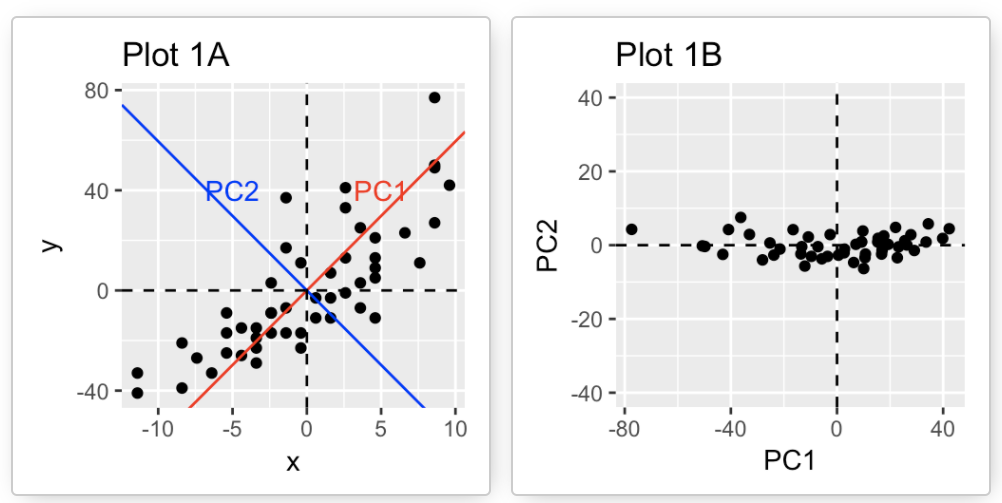
\includegraphics[width=0.6\textwidth,height=\textheight]{PCA_intro.png}
\caption{© Kassambara, 2017}
\end{figure}

\hypertarget{factor-analysis}{%
\section{Factor Analysis}\label{factor-analysis}}

Prior to PCA which has only become possible at the computer age, a related method was factor analysis, which was extensively applied to psychometric data. The aim of factor analysis is to summarize a set of variables by a smaller number of variables which helps in data interpretation. It is a linear statistical model, used to explain the variance among the observed variable and condense a set of the observed variable into the unobserved variable which is called factors (see the figure below). Factor analysis is on variables, not on individuals.

\begin{figure}
\centering
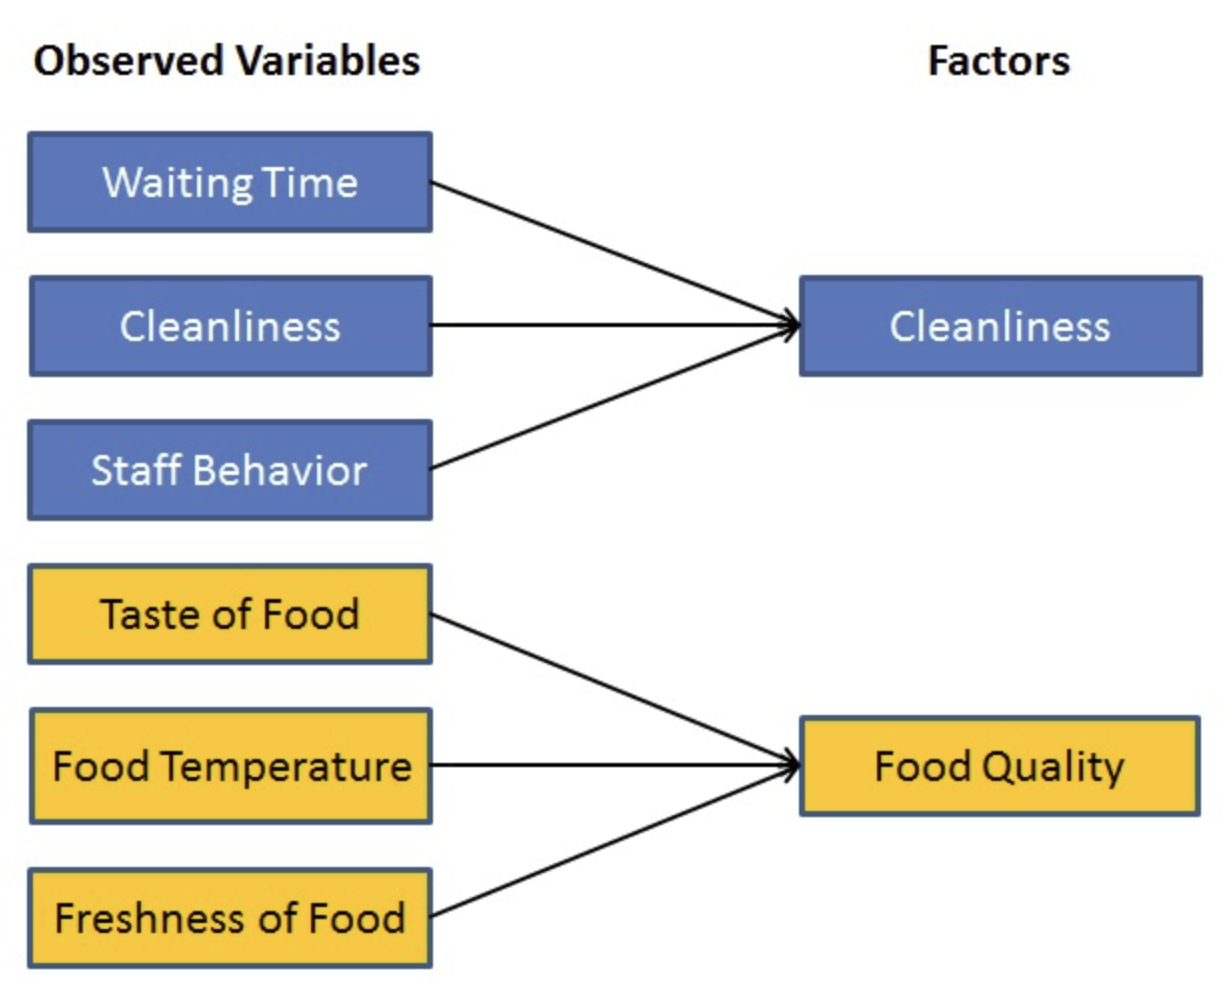
\includegraphics[width=0.5\textwidth,height=\textheight]{Factoranalysis.png}
\caption{© Navlani, 2019}
\end{figure}

\hypertarget{cluster-analysis}{%
\section{Cluster Analysis}\label{cluster-analysis}}

Cluster analysis is similar as PCA, one of the important methods for discovering knowledge in multidimensional data but differs since cluster analysis goes further to specify the characteristics of each sub-groups according to a defined distance measure.
Cluster analysis is applied in various fields of marketing, retail, medical science, sociology and so on.
The goal of clustering is to identify pattern or groups of similar objects within a dataset.
Following figure shows an example of cluster analysis of the states in the U.S. regarding arrested records.

\begin{Shaded}
\begin{Highlighting}[]
\KeywordTok{data}\NormalTok{(}\StringTok{"USArrests"}\NormalTok{)}
\NormalTok{df_a <-}\StringTok{ }\KeywordTok{scale}\NormalTok{(USArrests)}
\NormalTok{res.km <-}\StringTok{ }\KeywordTok{eclust}\NormalTok{(df_a, }\StringTok{"kmeans"}\NormalTok{, }\DataTypeTok{nstart =} \DecValTok{25}\NormalTok{)}
\end{Highlighting}
\end{Shaded}

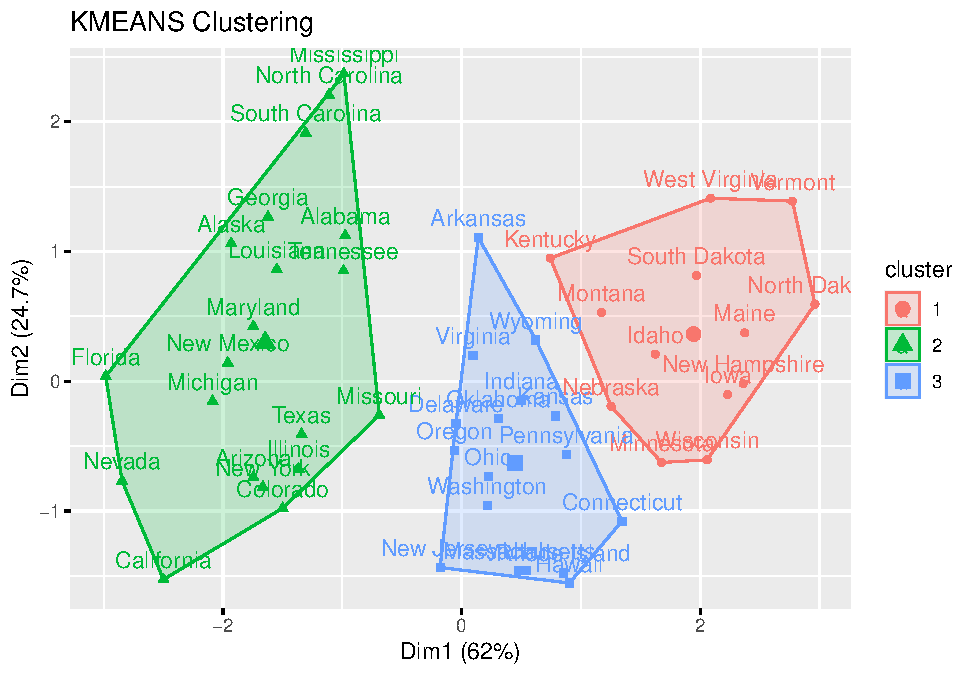
\includegraphics[width=0.6\linewidth]{Bookdown-MarinaObata2_files/figure-latex/1-2-1}

\hypertarget{correspondence-analysis-ca}{%
\section{Correspondence Analysis (CA)}\label{correspondence-analysis-ca}}

Correspondence analysis is the leading case of Geometric Data Analysis. CA is similar with PCA in the aspect of providing a solution for summarizing and visualizing data set into two-dimension plots, at the same time, as an extension of PCA, suited to explore among categorical data. CA is a geometric approach for visualizing the rows and columns of a two-way contingency table, in which positions of the row and column points are consistent with their association in the visualization. The goal of CA is to have a global view of the data that is useful for interpretation.
Following contingency table shows the data regarding division of housetasks in the couple, following graph visualizes the CA in the function of biplot, rows are represented by blue points and columns by red triangles.

\begin{figure}
\centering
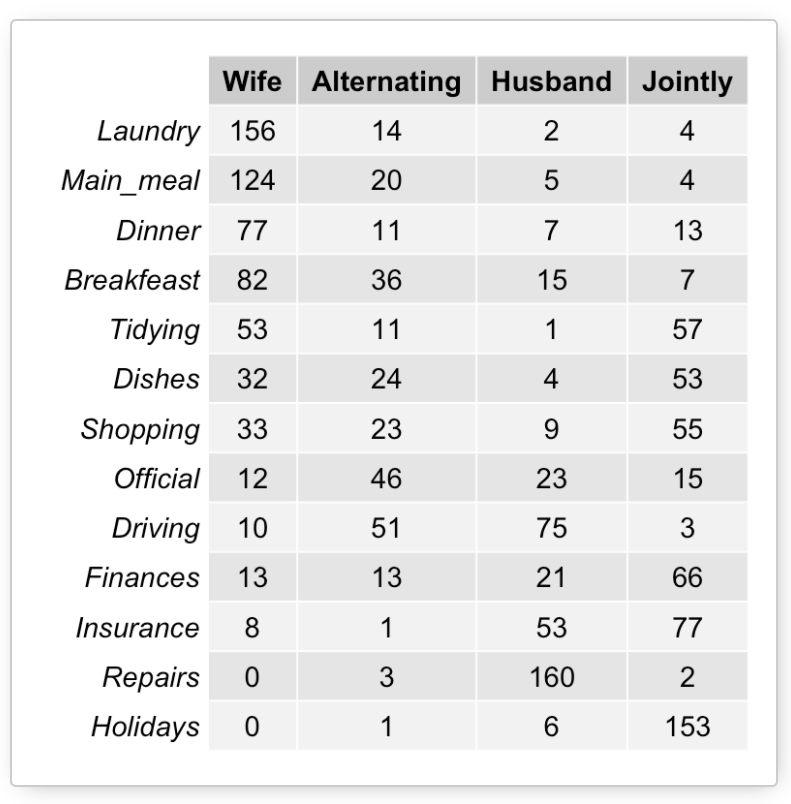
\includegraphics[width=0.55\textwidth,height=\textheight]{housework.png}
\caption{© Kassambara, 2017}
\end{figure}

\begin{Shaded}
\begin{Highlighting}[]
\KeywordTok{data}\NormalTok{(housetasks)}
\NormalTok{dt <-}\StringTok{ }\KeywordTok{as.table}\NormalTok{(}\KeywordTok{as.matrix}\NormalTok{(housetasks))}
\NormalTok{res.ca <-}\StringTok{ }\KeywordTok{CA}\NormalTok{(housetasks, }\DataTypeTok{graph =} \OtherTok{FALSE}\NormalTok{)}
\KeywordTok{fviz_ca_biplot}\NormalTok{(res.ca, }\DataTypeTok{repel =} \OtherTok{TRUE}\NormalTok{)}
\end{Highlighting}
\end{Shaded}

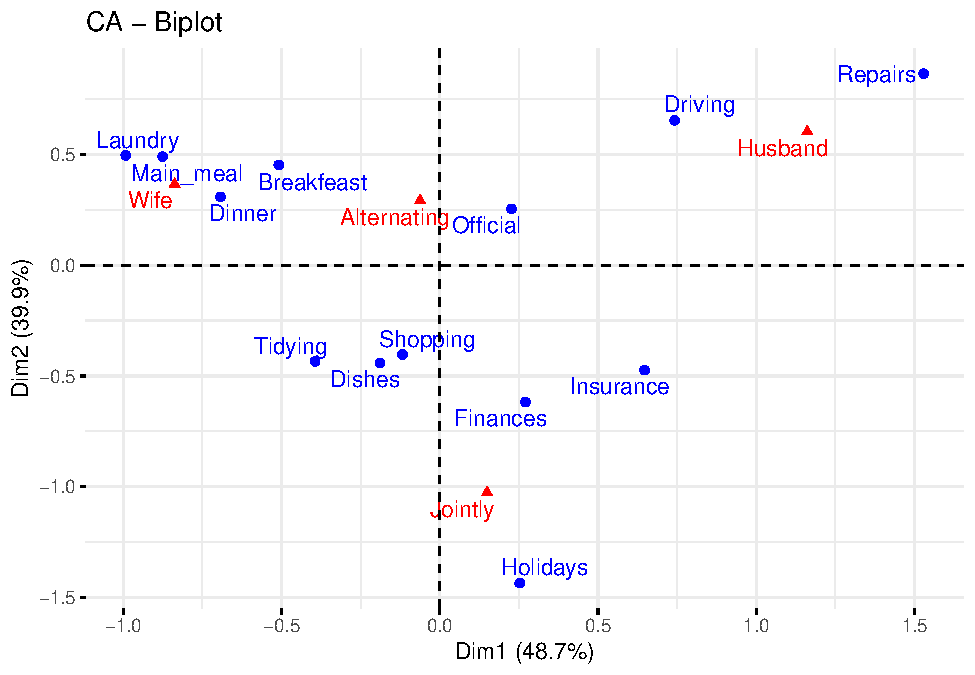
\includegraphics[width=0.6\linewidth]{Bookdown-MarinaObata2_files/figure-latex/1-3-1}

\hypertarget{eigenvalues}{%
\section{Eigenvalues}\label{eigenvalues}}

Eigenvalues are the values which won't be changed even the surface of the vector got moved in different directions. In PCA, eigenvalues measure the amount of variation retained by each principle component, in CA, eigenvalues correspond to the amount of information retained by each axis. Also, eigenvalues can be used to determine number of principal components/axis to be considered. In factor analysis, an eigenvalue is a measure of how much of the variance of the observed variables a factor explains.
The mathematics of eigenvalue is shown as following formula.

\begin{figure}
\centering
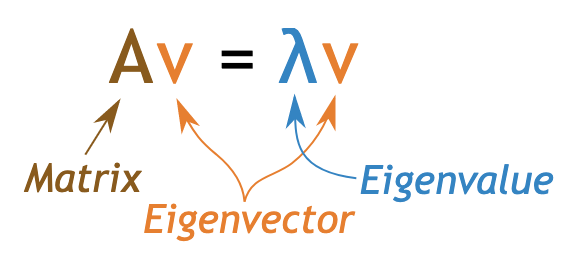
\includegraphics[width=0.5\textwidth,height=\textheight]{eigenvalue.png}
\caption{© MathsisFun, 2019}
\end{figure}

\hypertarget{eigenvectors}{%
\section{Eigenvectors}\label{eigenvectors}}

Eigenvectors are the vectors which won't change the directions even the surface of the vector got changed. Each eigenvector has a corresponding eigenvalue, if eigenvectors are sorted in descending order with respect to their eigen values, we will have the first eigenvector accounts for the largest spread among data, the second one for the second largest spread and so on.
In following example, the direction in green is the eigenvector, it has a corresponding eigenvalue which describes its magnitude.

\begin{figure}
\centering
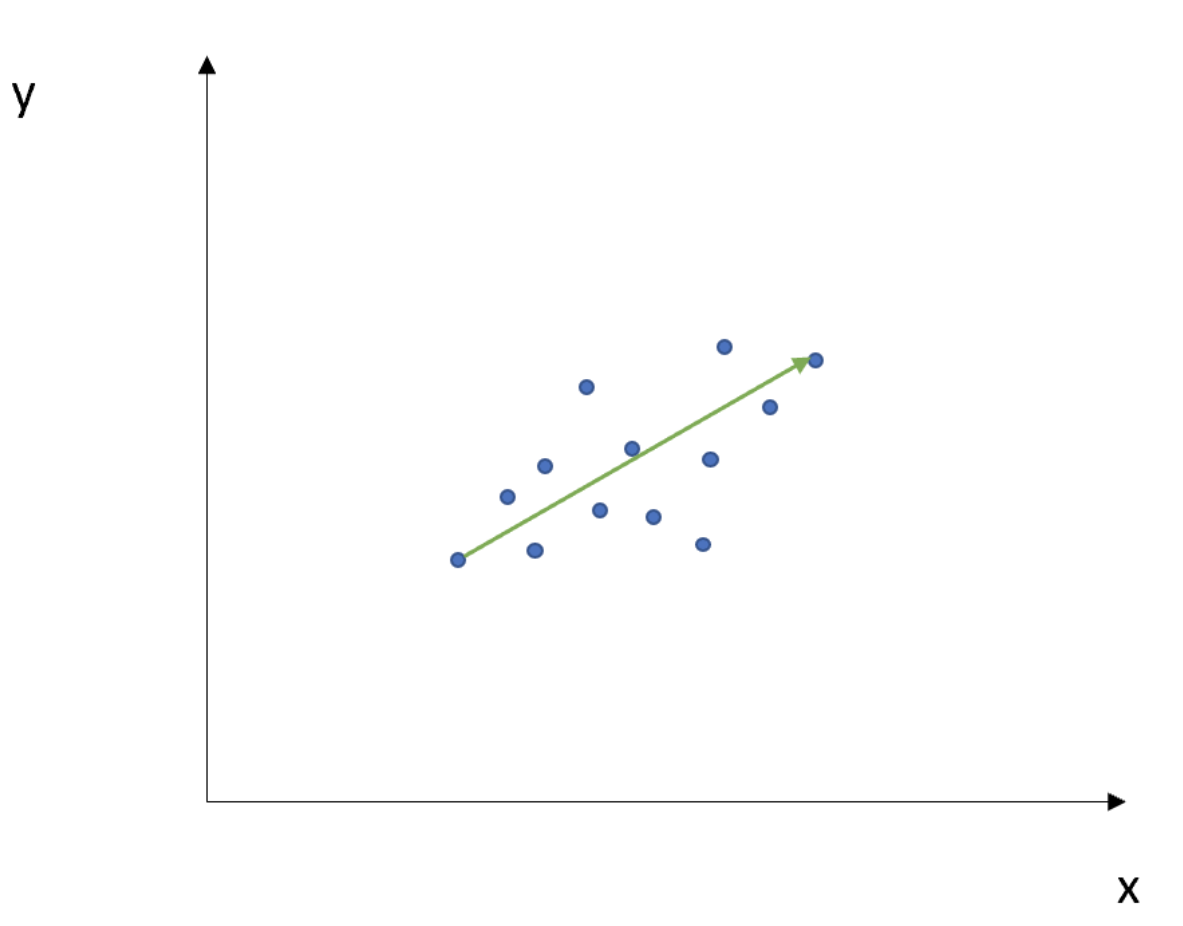
\includegraphics[width=0.5\textwidth,height=\textheight]{eigens.png}
\caption{© Alto, 2019}
\end{figure}

\hypertarget{variance}{%
\section{Variance}\label{variance}}

Variance shows how the group of the numbers are spreading around from its average.
If the variance has a large number, it means there is a large variation in numerical values within a group of the data. In PCA and CA, the large value of variance shows the importance, which means variance is showing the amount of information. Dimensions are ordered and listed accordingly to the amount of variance, dimension 1 explains the most variance, followed by dimension 2 and so on. Also, it is corresponding with the eigenvalue (see the table below.)

\begin{figure}
\centering
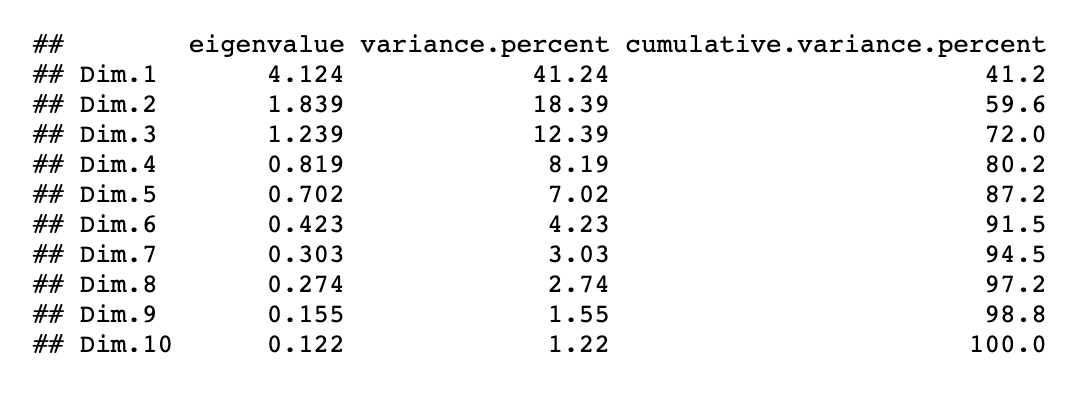
\includegraphics[width=0.7\textwidth,height=\textheight]{eigenvariance.png}
\caption{© Kassambara, 2017}
\end{figure}

\hypertarget{covariance}{%
\section{Covariance}\label{covariance}}

Covariance is the index which shows the relations of two variables. It is calculated as mean of deviations of two variables. As the value of covariance gets larger (in both positive and negative directions), which means that the correlation of two variables is strong, if the value is close to zero, which means there is almost no relations between two variables.
The following figure shows the shape of covariance matrix.
\[
{\sum =} \genfrac[]{0pt}{2}{Var(x) Cov(x,y)}{Cov(x,y) Var(y)} 
\]

\begin{figure}
\centering
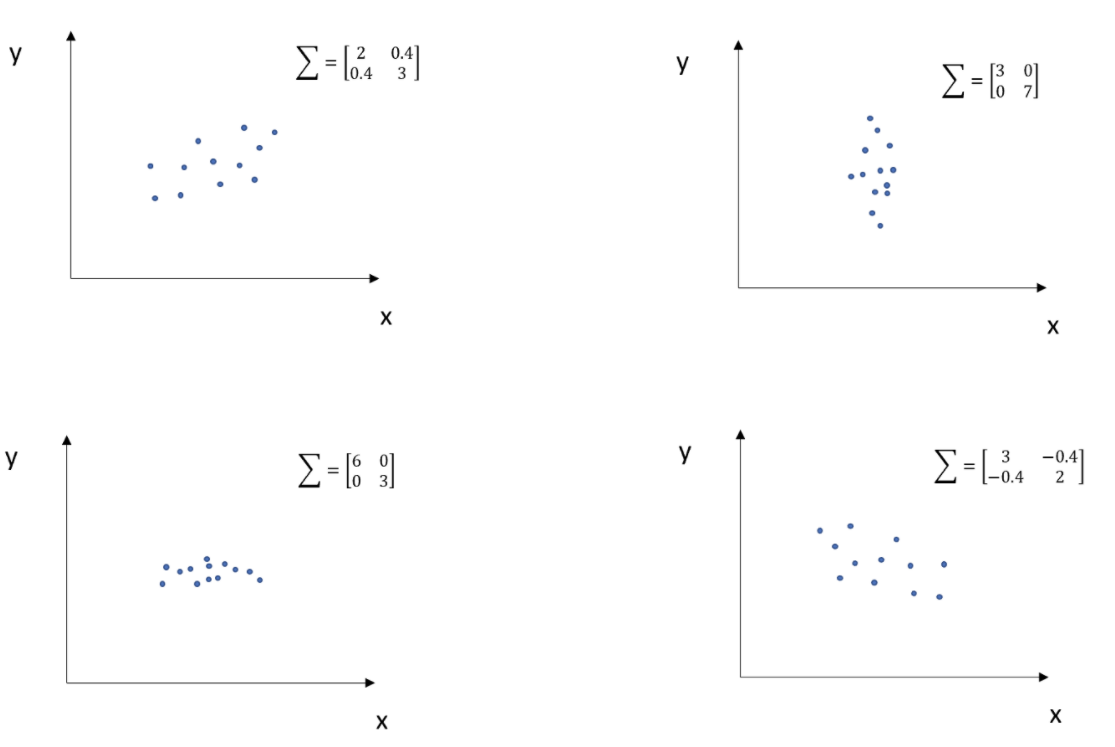
\includegraphics[width=0.6\textwidth,height=\textheight]{covariance.png}
\caption{© Alto, 2019}
\end{figure}

\hypertarget{references}{%
\section{References}\label{references}}

Alto.V.(2019).PCA: Eigenvectors and Eigenvalues. Towards data science. {[}online{]}.Retrieved from \url{https://towardsdatascience.com/pca-eigenvectors-and-eigenvalues-1f968bc6777a} {[}accessed on 14.06.2020{]}.

Garrett.G. and Wickham.H.(2017). R for Data science. O'Reilly.

Jolloffe.I. and Cadima.J. (2016). Principal component analysis: a review and recent developments. The royal society publishing.{[}online{]}.Retrieved from \url{https://royalsocietypublishing.org/doi/10.1098/rsta.2015.0202} {[}accessed on 14.06.2020{]}.

Kassambara.A. (2017). Articles - Principal Component Methods in R: Practical Guide. CA - Correspondence Analysis in R: Essentials. {[}online{]}. Retrieved from \url{http://www.sthda.com/english/articles/31-principal-component-methods-in-r-practical-guide/113-ca-correspondence-analysis-in-r-essentials/} {[}accessed on 15.06.2020{]}.

Kassambara.A. (2017). Practical Guide To Cluster Analysis in R. sthda.com . Edition 1.

Le Roux.B.and Rouanet.H. (2004). Geometric Data Analysis. Kluwer Academic Publishers.

MathsisFun (2019).Eigenvector and Eigenvalue. {[}online{]}.Retrieved from \url{https://www.mathsisfun.com/algebra/eigenvalue.html} {[}accessed on 14.06.2020{]}.

Navlani.A. (2019). Introduction to Factor Analysis in Python. DataCamp. {[}online{]}.Retrieved from \url{https://www.datacamp.com/community/tutorials/introduction-factor-analysis?utm_source=adwords_ppc\&utm_campaignid=898687156\&utm_adgroupid=48947256715\&utm_device=c\&utm_keyword=\&utm_matchtype=b\&utm_network=g\&utm_adpostion=\&utm_creative=229765585186\&utm_targetid=aud-299261629574:dsa-429603003980\&utm_loc_interest_ms=\&utm_loc_physical_ms=1003088\&gclid=EAIaIQobChMIoo7Oy_GB6gIViBsYCh2diAVmEAAYASAAEgIEUfD_BwE} {[} accessed on 15.06.2020{]}.

Patili.P. (2018).What is Exploratory Data Analysis? Towards Data Science. {[}online{]}. Retrieved from \url{https://towardsdatascience.com/exploratory-data-analysis-8fc1cb20fd15\%5Baccessed} on 14.06.2020{]}.

Rahn.M.Factor Analysis: A Short Introduction, Part 1. The analysis factor.{[}online{]}.Retrieved from \url{https://www.theanalysisfactor.com/factor-analysis-1-introduction/\#}:\textasciitilde{}:text=In\%20every\%20factor\%20analysis\%2C\%20there,factors\%20as\%20there\%20are\%20variables.\&text=The\%20eigenvalue\%20is\%20a\%20measure,than\%20a\%20single\%20observed\%20variable.{[}accessed on 16.07.2020{]}.

\hypertarget{glossary-2-pca}{%
\chapter{Glossary 2 (PCA)}\label{glossary-2-pca}}

\hypertarget{cloud-of-variables}{%
\section{Cloud of variables}\label{cloud-of-variables}}

In Geometric Data Analysis(GDA), there are three main paradigms, which are Simple Correspondence Analysis(CA), studies contingency tables, Principle Component Analysis(PCA), studies Individuals x Numerical variables tables and Multiple Correspondence Analysis (MCA), studies Individuals x Categorical variables tables.
In GDA, cloud of plots are built using numerical data sets. In PCA, cloud of variables includes not only the elements from majour variables, but also supplementary elements.
The cloud of variables is a representation of the associations between variables which can be quantified by linear correlation coefficient, it can be defined by a set of vectors starting from the center, the correlation coefficient characterizes the angle.
It is explained as following image.

\begin{figure}
\centering
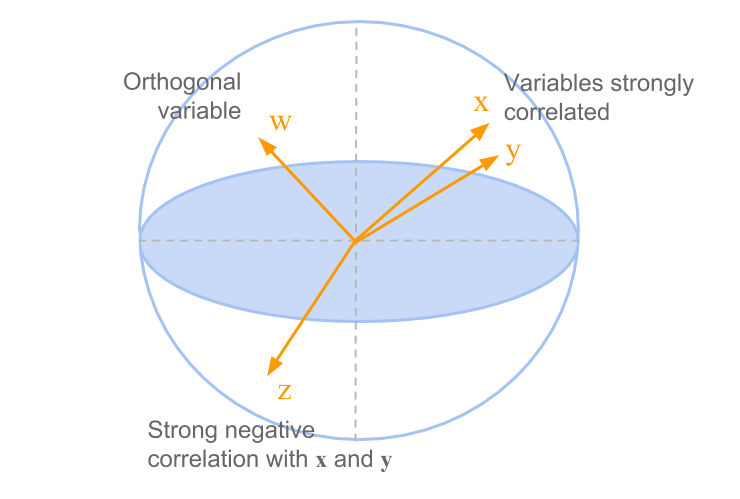
\includegraphics[width=0.5\textwidth,height=\textheight]{Figure_variable.png}
\caption{© Aluja-Banet.T. et al(2019).}
\end{figure}

\hypertarget{cloud-of-individuals}{%
\section{Cloud of individuals}\label{cloud-of-individuals}}

Cloud of individuals are also related to GDA in PCA, MCA and CA. Cloud of individuals can be considered as cloud of row-points, more related to individual factors (i.e.~Country, Person, Genes etc..).
Cloud of individuals can contribute to the systematical analysis in especially economic field research in combination with more qualitative methods since it enables us to investigate the empirical description of all relevant actors in the particular social space.
The following example shows the cloud of individuals in PCA, as we can see, it also indicates how strong individuals are contributing. Additionally, it enables to observe the outliers and individuals having similar characteristics.

\begin{figure}
\centering
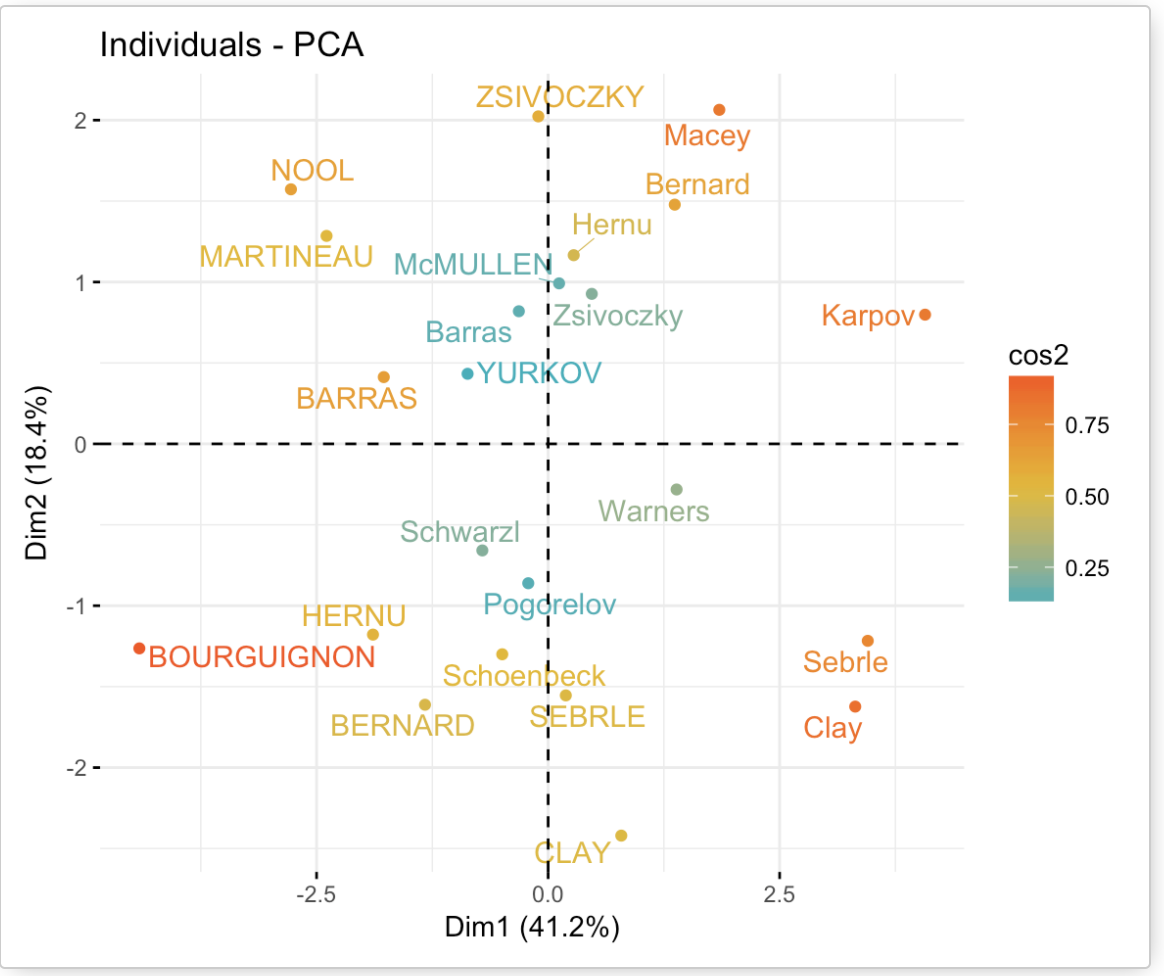
\includegraphics[width=0.5\textwidth,height=\textheight]{individuals.png}
\caption{© Kassambara (2017).}
\end{figure}

\hypertarget{principal-component}{%
\section{Principal Component}\label{principal-component}}

When we want to analyse the data which has cloud of the observations, spreading by the variables and individuals, principal component helps to find the structure of the clouds.
Principal component is the line which goes between the points composing the swarm to where the data variation is maximized. Also, passes through the central point of the cloud. It is an important information from a multivariate data table, expressing the information as a set of few new variables.
From each point of spread observations, the relations between the drawn principal component is 90 degrees of straight line (see the image below.)
Moreover, in case of the first principal line is not explaining the other variables well, by repeating this projection procedure, several more principal component can be found.

\begin{figure}
\centering
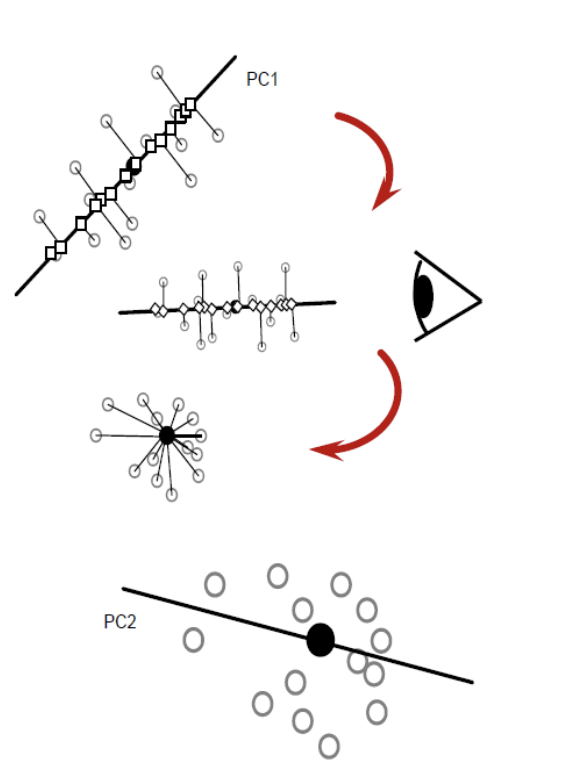
\includegraphics[width=0.5\textwidth,height=\textheight]{PC1_2.png}
\caption{© image by Joon}
\end{figure}

\hypertarget{active-variables}{%
\section{Active variables}\label{active-variables}}

Active variables are the variables which may have important influences on the structure of the point clouds. Also, it is directly connected with the research question of what to be examined in the survey. Among variables, active variables will serve to define the distances between individuals.
In the example below, active variables are subset from whole variables of the dataset `decathlon'. Which means that in this dataset, these variables are having influences on the structure.

\begin{Shaded}
\begin{Highlighting}[]
\KeywordTok{data}\NormalTok{(decathlon2)}
\NormalTok{decathlon2.active <-}\StringTok{ }\NormalTok{decathlon2[}\DecValTok{1}\OperatorTok{:}\DecValTok{23}\NormalTok{, }\DecValTok{1}\OperatorTok{:}\DecValTok{10}\NormalTok{]}
\KeywordTok{head}\NormalTok{(decathlon2.active[, }\DecValTok{1}\OperatorTok{:}\DecValTok{6}\NormalTok{], }\DecValTok{4}\NormalTok{)}
\end{Highlighting}
\end{Shaded}

\begin{verbatim}
##         X100m Long.jump Shot.put High.jump X400m X110m.hurdle
## SEBRLE  11.04      7.58    14.83      2.07 49.81        14.69
## CLAY    10.76      7.40    14.26      1.86 49.37        14.05
## BERNARD 11.02      7.23    14.25      1.92 48.93        14.99
## YURKOV  11.34      7.09    15.19      2.10 50.42        15.31
\end{verbatim}

\hypertarget{supplementary-variables}{%
\section{Supplementary variables}\label{supplementary-variables}}

Supplementary variables can also be called as ``passive variables''. Compared to active variables, they are not directory influencing on the structure. However, they have variety of analytic possibilities, it helps to distinguish certain groups of individuals by integrating ANOVA analysis. By doing so, supplementary variables can find correlation of themselves in the space constructed by active variables.
As an example, the study which researched about life style and consumption from the point of view of groups and interests, the active variables were set as question on tastes and cultural practices, the variables of socio-demographic and occupation were set as supplementary variables.
Another example below is showing continuously the dataset of `decathlon' from 3.4'active variables', the variables shown in red are indicating the supplementary variables, which are `rank' and `points' of athletes, in contrast to the active variables showing the name of events.

\begin{Shaded}
\begin{Highlighting}[]
\KeywordTok{data}\NormalTok{(decathlon2)}
\NormalTok{res.pca2 <-}\StringTok{ }\KeywordTok{PCA}\NormalTok{(decathlon2, }\DataTypeTok{ind.sup =} \DecValTok{24}\OperatorTok{:}\DecValTok{27}\NormalTok{, }
               \DataTypeTok{quanti.sup =} \DecValTok{11}\OperatorTok{:}\DecValTok{12}\NormalTok{, }\DataTypeTok{quali.sup =} \DecValTok{13}\NormalTok{, }\DataTypeTok{graph=}\OtherTok{FALSE}\NormalTok{)}
\KeywordTok{fviz_pca_var}\NormalTok{(res.pca2,}
             \DataTypeTok{col.var =} \StringTok{"black"}\NormalTok{,     }
             \DataTypeTok{col.quanti.sup =} \StringTok{"red"} 
\NormalTok{             )}
\end{Highlighting}
\end{Shaded}

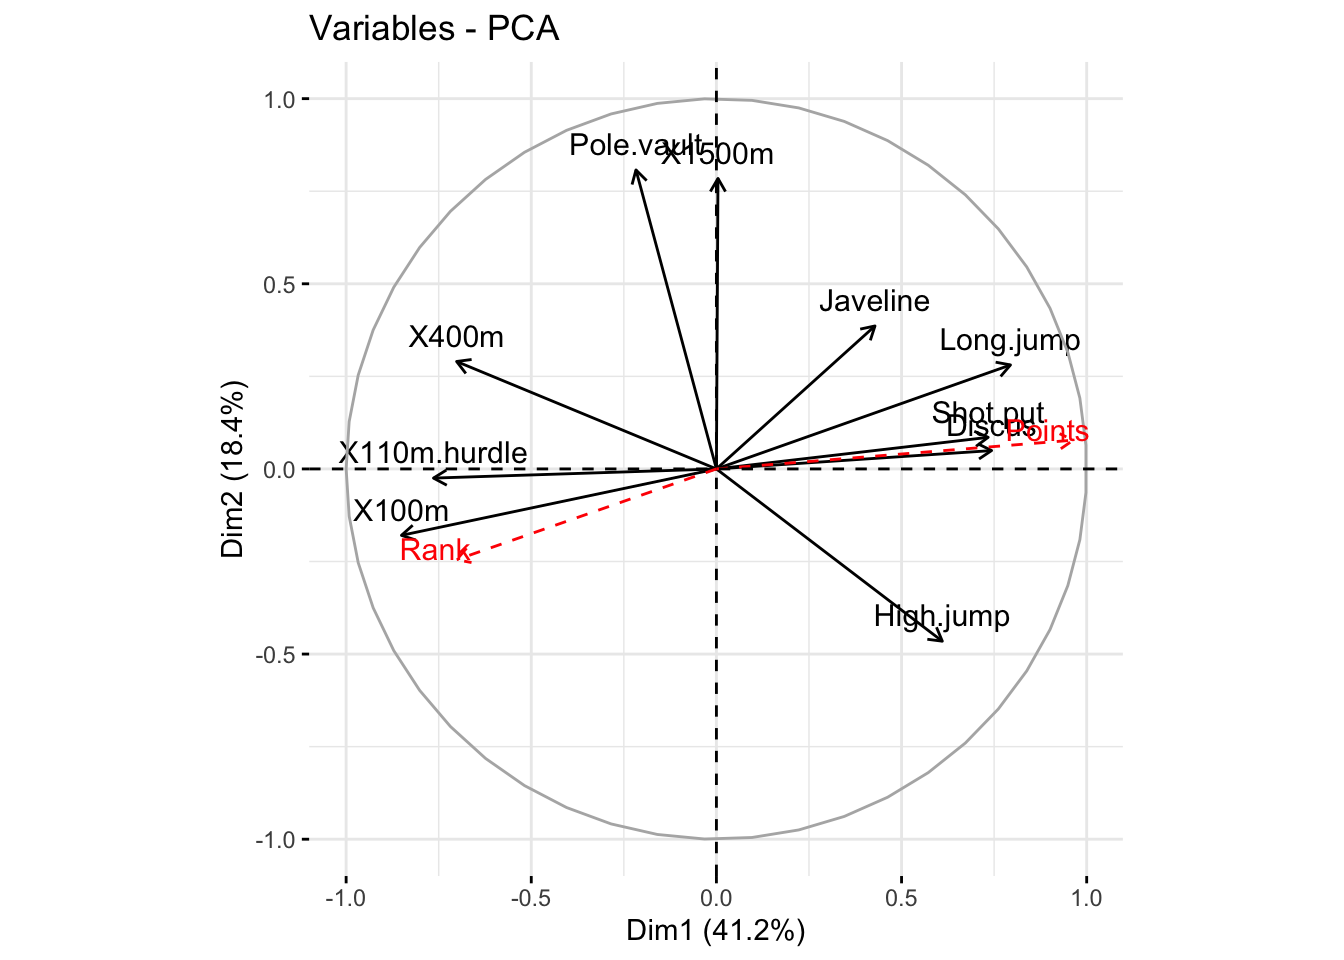
\includegraphics[width=0.6\linewidth]{Bookdown-MarinaObata2_files/figure-latex/2-3-1}

\hypertarget{eigenvalues-interpretation-in-factor-analysis-and-principal-component-analysis}{%
\section{Eigenvalues (interpretation in Factor Analysis and Principal Component Analysis)}\label{eigenvalues-interpretation-in-factor-analysis-and-principal-component-analysis}}

Eigenvalues express the total amount of variance which can be explained by a principal component. If the eigenvalue is close to zero, multicollinearity must be doubted. In factor analysis, eigenvalues can be the indicator of factor; if it has low values, it means less importance than the factors with higher values since it is related to the explanatory abilities towards variances in variables.
In PCA, the eigenvalues of correlation represent the ``core'' of PCA, it explains the degree of the variance of the data along with the new axis of principal component to be created.

\hypertarget{rotation}{%
\section{Rotation}\label{rotation}}

Rotation means a movement of an axis which goes between cloud of points. This cloud of points can be considered as group of rotation here. The point which stays the same in any dimension in rotation is called as center of rotation (the green point in the image). As the group rotates, the variance of the axis changes, the best fit would be when axis's rotation stops where the variance shows the largest value. In GDA, it is better to doubt the homogeneity of the data when a rotation of one of the first axis occurs.

\begin{figure}
\centering
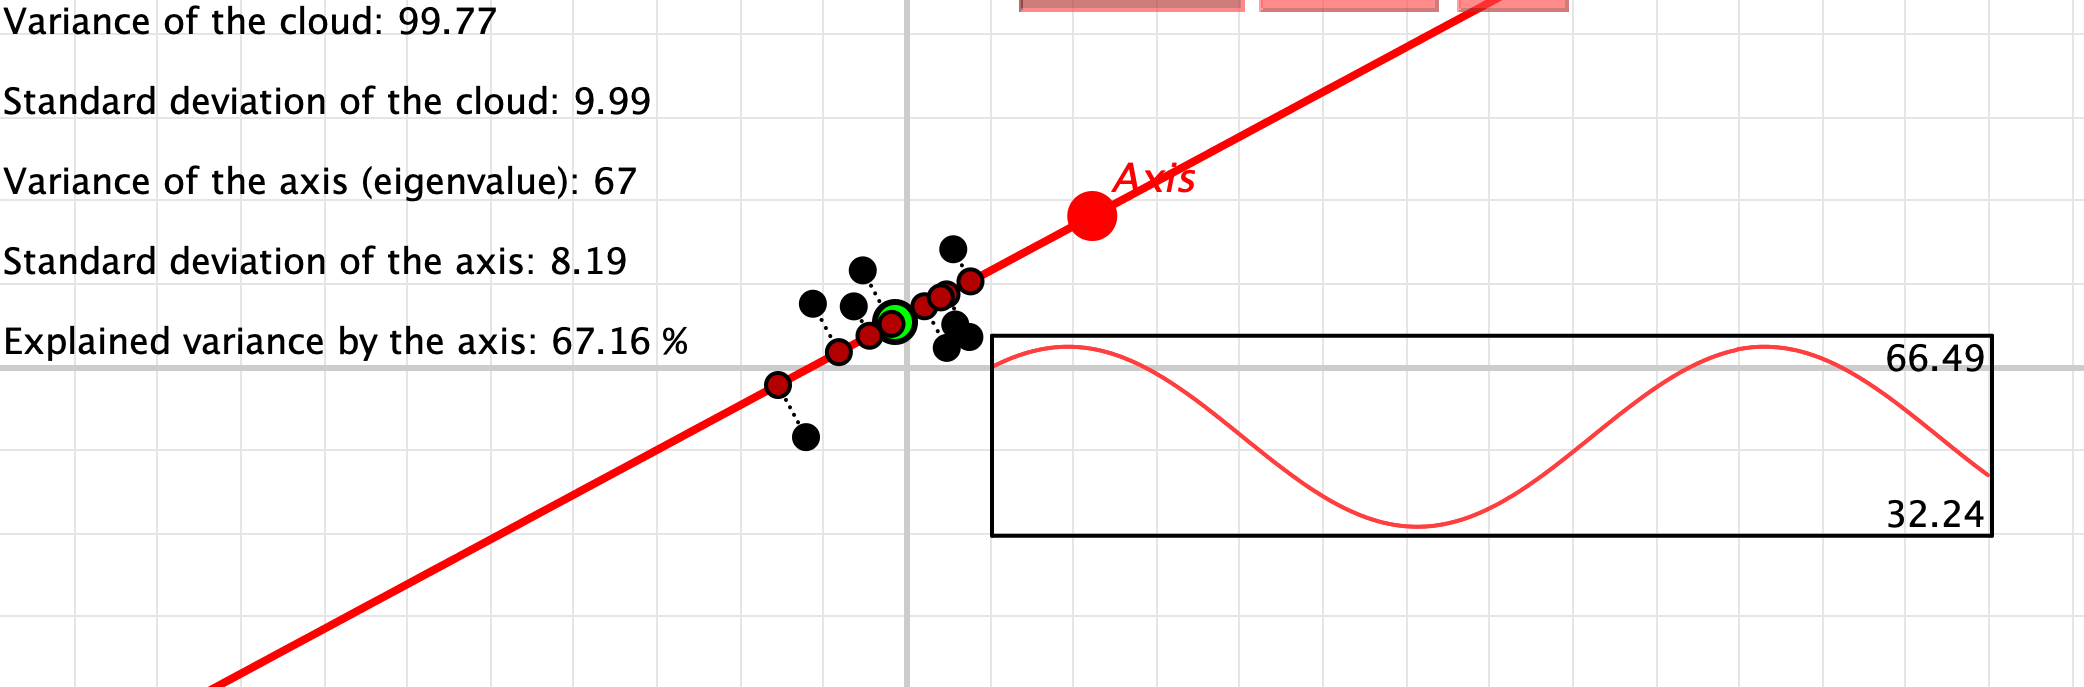
\includegraphics[width=0.6\textwidth,height=\textheight]{Rotation.png}
\caption{© Cinderella image}
\end{figure}

\hypertarget{screeplot}{%
\section{Screeplot}\label{screeplot}}

As an alternative method to determine the number of principal components apart from eigenvalues is to look at scree plot. Screeplot displays the cumulative variance explained by each principal component in descending order. A good solution to determine the number of components might be the point which screeplot displays an `elbow', in case the `elbow' is not observable, as a rule of thumb, more than 70 percent of cumulative number of explained variance is a good value to judge.
From the example of the dataset `decathlon', following figure shows its scree plot.

\begin{Shaded}
\begin{Highlighting}[]
\KeywordTok{fviz_eig}\NormalTok{(res.pca2, }\DataTypeTok{addlabels =} \OtherTok{TRUE}\NormalTok{, }\DataTypeTok{ylim =} \KeywordTok{c}\NormalTok{(}\DecValTok{0}\NormalTok{, }\DecValTok{50}\NormalTok{))}
\end{Highlighting}
\end{Shaded}

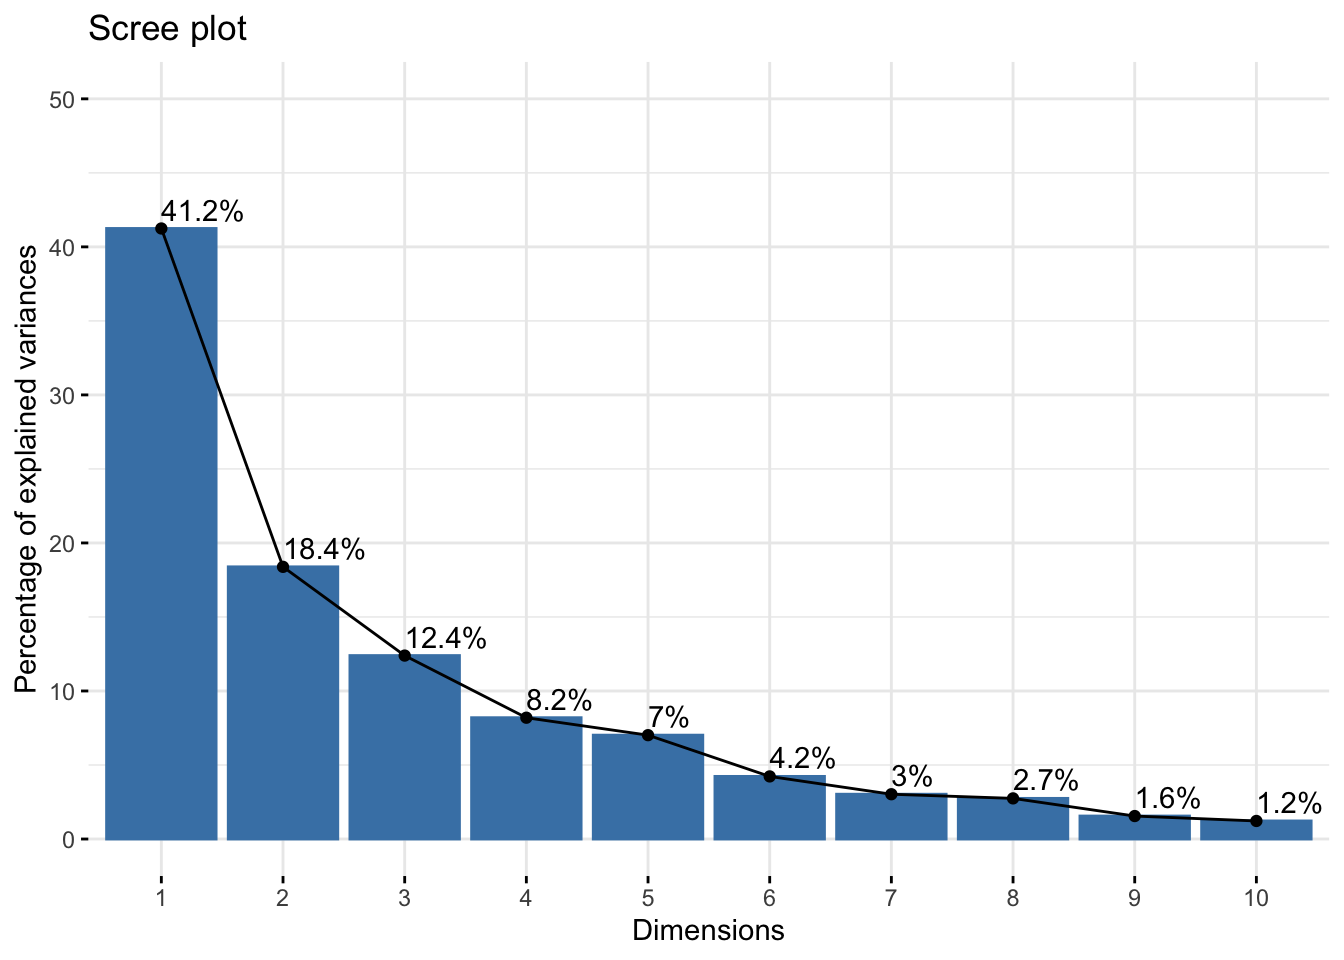
\includegraphics[width=0.6\linewidth]{Bookdown-MarinaObata2_files/figure-latex/2-4-1}

\hypertarget{references-1}{%
\section{References}\label{references-1}}

Auja-Banet.T., Morineau.A. and Sanchez.G.(2018). Principal Component Analysis for Data Science (pca4ds). {[}online{]}.Retrieved from \url{https://pca4ds.github.io/index.html} {[}accessed on 15.06.2020{]}.

Jolloffe.I. and Cadima.J. (2016). Principal component analysis: a review and recent developments. The royal society publishing.{[}online{]}.Retrieved from \url{https://royalsocietypublishing.org/doi/10.1098/rsta.2015.0202} {[}accessed on 14.06.2020{]}

Kassambara.A. (2017).Articles - Principal Component Methods in R: Practical Guide. Principal Component Analysis in R: prcomp vs princomp. {[}online{]}.Retrieved from \url{http://www.sthda.com/english/articles/31-principal-component-methods-in-r-practical-guide/118-principal-component-analysis-in-r-prcomp-vs-princomp/} {[}accessed on 15.06.2020{]}.

Le Roux.B.and Rouanet.H. (2004). Geometric Data Analysis. Kluwer Academic Publishers.

Image source: Joon.Y. Principal Component Analysis. {[}online{]}.Retrieved from \url{https://www.cheric.org/files/education/cyberlecture/d201401/d201401-601.pdf} {[}accessed on 22.03.2020{]}.

\hypertarget{glossary-3-factor-analysis}{%
\chapter{Glossary 3 (Factor Analysis)}\label{glossary-3-factor-analysis}}

\hypertarget{factor}{%
\section{Factor}\label{factor}}

Factor is a classified element from which it is being a cause in general, in factor analysis, factor means the underlying variables which is smaller than the observed variables, explains how those observed variables are interrelated each other.
Factor analysis is aiming to model the interrelationships among items which is explained by the found factors. The relation between observed variables and factors are shown in following image.

\begin{figure}
\centering
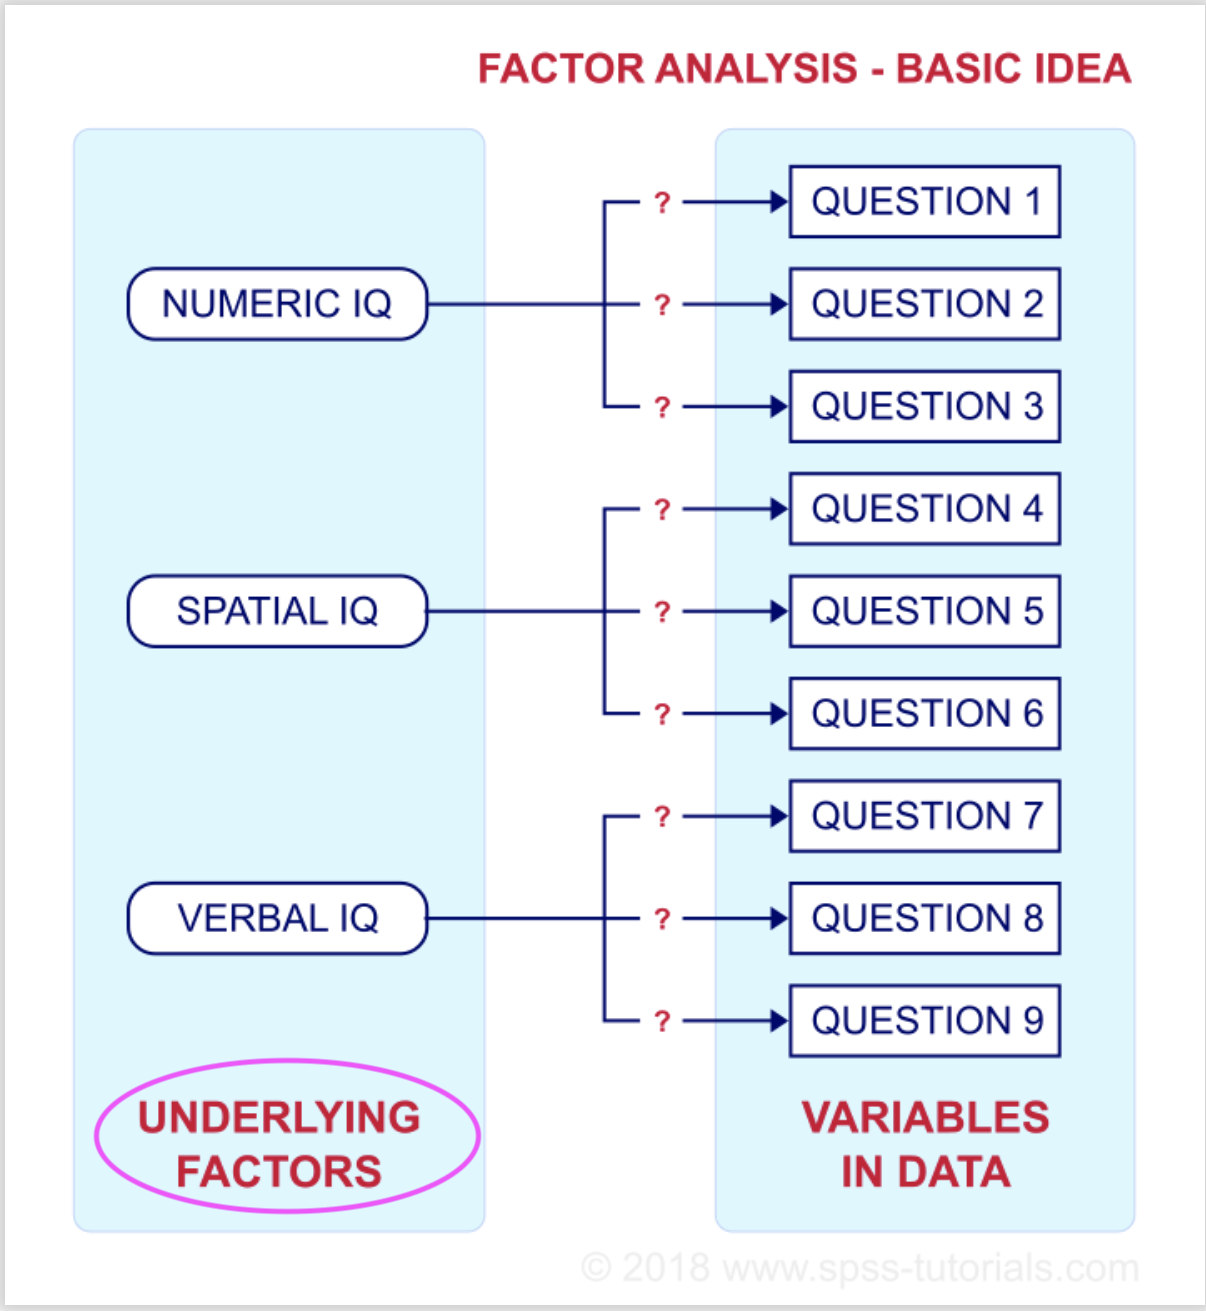
\includegraphics[width=0.4\textwidth,height=\textheight]{Factor.png}
\caption{© van den Berg}
\end{figure}

\hypertarget{communalities}{%
\section{Communalities}\label{communalities}}

Communality describes a common variance which ranges between 0 and 1 in factor analysis, symbol of communality is shown as h\^{}2 (see the notation below). The common variance is the shared variance among the items, as more these items are strongly related from each other, shared variance gets larger. Communalities give how well the model performs, if communality is closer to 1, it means that the extracted factors by the analysis explain more variance of an item. In that case, the model explains better. The total variance in factor analysis is consisted from common variance and unique variance which is composed of specific(S) and error(E) variance (see image below).The individual communarities tell how it is explained for individual variables, overall communarities gives an overall assessment of the performance.

\[
\hat{h}_i^2 = {\sum_{j=1}^m} \hat{l}_{ij}^2
\]

\begin{figure}
\centering
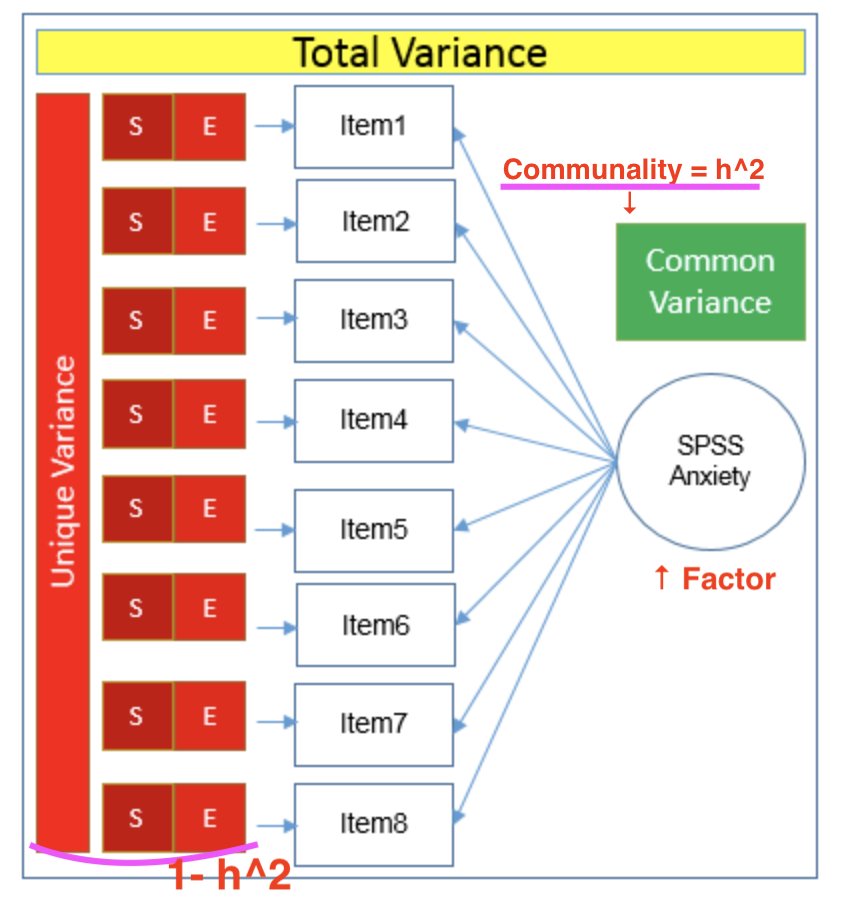
\includegraphics[width=0.4\textwidth,height=\textheight]{Communality.png}
\caption{© UCLA.}
\end{figure}

In comparison, in PCA, the communality is the sum of extracted proportion of variance of selected components.In PCA, unique variance is not taken into account. Thus, if the communalities across all items are summed up, it is equal to total variance. The sum of eigenvalues of each component is also equal to the total variance, therefore, those communalities and eigenvalues are equal in PCA.
When the total variance is 1, then common variance = communality.

\hypertarget{factor-loadings}{%
\section{Factor loadings}\label{factor-loadings}}

Factor loadings are the correlation coefficients between the variables and factors in factor analysis and PCA. It shows how much the variance in the variable is explained by the factor. Loadings can be between -1 to 1, close to -1 and 1 means that the factor influences strongly towards the variable, close to 0 means the influence is weak.
If a variable has more than one significant factor loadings, it is called as cross loadings which is hard to interpret. In this case, rotation of factor loadings is proceeded, so that the factor loadings are redistributed as each variable measures only one factor.
Following example shows the solution of factor loadings of data ``Thurstone'' between factors (RC1-RC3) and variables which are indicating the ability items.

\begin{Shaded}
\begin{Highlighting}[]
\KeywordTok{data}\NormalTok{(Thurstone)}
\NormalTok{fa3 <-}\StringTok{ }\KeywordTok{principal}\NormalTok{(}\DataTypeTok{r =}\NormalTok{ Thurstone,}
  \DataTypeTok{nfactors =} \DecValTok{3}\NormalTok{,}
  \DataTypeTok{n.obs =} \DecValTok{213}\NormalTok{)}
\KeywordTok{print}\NormalTok{(fa3}\OperatorTok{$}\NormalTok{loadings, }\DataTypeTok{cutoff=}\DecValTok{0}\NormalTok{, }\DataTypeTok{digits=}\DecValTok{3}\NormalTok{)}
\end{Highlighting}
\end{Shaded}

\begin{verbatim}
## 
## Loadings:
##                   RC1   RC2   RC3  
## Sentences         0.863 0.243 0.229
## Vocabulary        0.854 0.314 0.189
## Sent.Completion   0.849 0.262 0.189
## First.Letters     0.226 0.823 0.231
## Four.Letter.Words 0.183 0.791 0.301
## Suffixes          0.314 0.773 0.057
## Letter.Series     0.249 0.158 0.834
## Pedigrees         0.534 0.080 0.613
## Letter.Group      0.095 0.311 0.805
## 
##                  RC1   RC2   RC3
## SS loadings    2.735 2.254 1.990
## Proportion Var 0.304 0.250 0.221
## Cumulative Var 0.304 0.554 0.775
\end{verbatim}

\hypertarget{factor-values-factor-scores}{%
\section{Factor values (Factor scores)}\label{factor-values-factor-scores}}

When factor loadings are low, or looks very different from each other, it is possible to create an index which reflects the inequality of association between items and the factor, which are the factor scores. Factor scores are the estimated values of factors, optimally weighted linear combination of the items, creating the index variable. Each item's weight is derived from its factor loading, thus, each item's contribution to the factor score depends on how strongly it relates to the factor. The reason why factor scores are essentially weighted sum of the items is that those weights are between -1 to 1, the scale of the factor scores would be varied from a pure sum.

\hypertarget{anti-image-correlation-matrix}{%
\section{Anti-image correlation matrix}\label{anti-image-correlation-matrix}}

Anti-image is a part of variable which cannot be predicted, since the image of a variable is defined as a part which is predictable by regressing each variables. Anti-image correlation matrix indicates how the items are correlated in the matrix, it summarizes the most important information about partial correlations. Thus, helping to indicate the part of variables which is not predictable. The diagonal values are the KMO(explained later) measures of sampling adequacy, the off-diagonal values are showing the negative of the pairwise partial correlation coefficients. Most of the off-diagonal elements should be small so that the factor analysis model can be considered as having better goodness.
Following figure is showing the example from the data of ``Thurstone''.

\begin{Shaded}
\begin{Highlighting}[]
\KeywordTok{cor}\NormalTok{(Thurstone, }\DataTypeTok{use=}\StringTok{"pairwise"}\NormalTok{)}
\end{Highlighting}
\end{Shaded}

\begin{verbatim}
##                    Sentences  Vocabulary Sent.Completion First.Letters
## Sentences          1.0000000  0.91636022      0.86759906    -0.3041112
## Vocabulary         0.9163602  1.00000000      0.86863779    -0.1784238
## Sent.Completion    0.8675991  0.86863779      1.00000000    -0.2315780
## First.Letters     -0.3041112 -0.17842378     -0.23157804     1.0000000
## Four.Letter.Words -0.3652704 -0.27790681     -0.33725544     0.6607587
## Suffixes          -0.1322282 -0.02188666     -0.09780351     0.4881992
## Letter.Series     -0.2355010 -0.32712116     -0.32540886    -0.4848485
## Pedigrees          0.2202801  0.15769908      0.19825849    -0.6161762
## Letter.Group      -0.4856669 -0.57378661     -0.52569295    -0.2543441
##                   Four.Letter.Words    Suffixes Letter.Series   Pedigrees
## Sentences                -0.3652704 -0.13222821    -0.2355010  0.22028010
## Vocabulary               -0.2779068 -0.02188666    -0.3271212  0.15769908
## Sent.Completion          -0.3372554 -0.09780351    -0.3254089  0.19825849
## First.Letters             0.6607587  0.48819920    -0.4848485 -0.61617617
## Four.Letter.Words         1.0000000  0.35087898    -0.3811472 -0.55819512
## Suffixes                  0.3508790  1.00000000    -0.6777077 -0.58649627
## Letter.Series            -0.3811472 -0.67770771     1.0000000  0.32820549
## Pedigrees                -0.5581951 -0.58649627     0.3282055  1.00000000
## Letter.Group             -0.1476621 -0.49914387     0.5042140 -0.01395292
##                   Letter.Group
## Sentences          -0.48566690
## Vocabulary         -0.57378661
## Sent.Completion    -0.52569295
## First.Letters      -0.25434412
## Four.Letter.Words  -0.14766210
## Suffixes           -0.49914387
## Letter.Series       0.50421396
## Pedigrees          -0.01395292
## Letter.Group        1.00000000
\end{verbatim}

\hypertarget{kaiser-meyer-olkin-criterion-kmo}{%
\section{Kaiser-Meyer-Olkin criterion (KMO)}\label{kaiser-meyer-olkin-criterion-kmo}}

Kaiser-Meyer-Olkin criterion (KMO) is a modified version of the Measure of Sampling Adequacy (MSA, will be explained below), by Kaiser and Rice (1974). It indicates the degree of each variables in a dataset can be predicted without error which caused by other variables. This analysis is relying on anti-image correlation matrix, measured by 0 to 1, value 0 means that the sum of partial correlation is large compared to the sum of correlations which means the correlations are wide spread, this is indicating the factor analysis is not likely be appropriate. Thus, if the value is closer to 1, the dataset is considered as suitable for factor analysis.
Mathematical notation is as follows.
\[
KMO =  \frac {\sum_{i=1}^k \sum_{j=1}^k r_{ij}^2} {\sum_{i=1}^k \sum_{j=1}^k r_{ij}^2 + a_{ij}^2} ,   i\ne j
\]

\hypertarget{measure-of-sampling-adequacy-msa}{%
\section{Measure of Sampling Adequacy (MSA)}\label{measure-of-sampling-adequacy-msa}}

Measure of Sampling Adequacy (MSA) is introduced by Kaiser(1970) before he modified Kaiser Meyer-Olkin criterion. This is a statistical value used as an index for deciding if the sample is suitable for performing factor analysis or not. It calculates the measure of 0 to 1, as the result is closer to 1, it is better, 0.6 is the suggested minimum. It is mentioned that MSA increases 1)when the number of variables increases, 2)when the effective number of factors increases, 3)when the overall level of correlation increases, and 4)when sample size of individuals increases.
Mathematical notation is as follows.

\[
MSA_i =  \frac {\sum_{j=1}^k r_{ij}^2} {\sum_{j=1}^k r_{ij}^2 + a_{ij}^2} ,   j \ne i
\]

Given these explanation, KMO has been applied to the data of ``Thurstone''.

\begin{Shaded}
\begin{Highlighting}[]
\KeywordTok{KMO}\NormalTok{(Thurstone)}
\end{Highlighting}
\end{Shaded}

\begin{verbatim}
## Kaiser-Meyer-Olkin factor adequacy
## Call: KMO(r = Thurstone)
## Overall MSA =  0.88
## MSA for each item = 
##         Sentences        Vocabulary   Sent.Completion     First.Letters 
##              0.86              0.86              0.90              0.86 
## Four.Letter.Words          Suffixes     Letter.Series         Pedigrees 
##              0.88              0.92              0.85              0.93 
##      Letter.Group 
##              0.87
\end{verbatim}

Considering the value, overall value and all of values for each item are higher than 0.6, very close to 1, it can be assumed that the data is suitable for factor analysis.

\hypertarget{references-2}{%
\section{References}\label{references-2}}

Cerny.B.A. and Kaiser.H.F.(2010). A Study Of A Measure Of Sampling Adequacy For Factor-Analytic Correlation Matrices. Taylor \& Francis Online. {[}online{]}.Retrieved from \url{https://www.tandfonline.com/doi/abs/10.1207/s15327906mbr1201_3} {[}accessed on 15.06.2020{]}.

Lüdecke.D., Makowski.D.and Mattan.S.B.S. Kaiser, Meyer, Olkin (KMO) Measure of Sampling Adequacy (MSA) for Factor Analysis.{[}online{]}.Retrieved from \url{https://easystats.github.io/parameters/reference/check_kmo.html} {[}accessed on 15.06.2020{]}.

Le Roux.B.and Rouanet.H. (2004). Geometric Data Analysis. Kluwer Academic Publishers.

PennEtate Eberly College of Science. (2020).12.5 - Communalities. The Pennsylvania State University. {[}online{]}. Retrieved from \url{https://online.stat.psu.edu/stat505/lesson/12/12.5} {[}accessed on 16.06.2020{]}.

Quicl.J. M. (2014). R Tutorial Series. {[}online{]}.Retrieved from \url{http://rtutorialseries.blogspot.com/2011/10/r-tutorial-series-exploratory-factor.html} {[}accessed on 15.06.2020{]}.

Revelle. W.(2019). How To: Use the psych package for Factor Analysis and data reduction. Department of Psychology
Northwestern University. {[}online{]}. Retrieved from \url{http://personality-project.org/r/psych/HowTo/factor.pdf} {[}accessed on 15.06.2020{]}

Revelle. W.(2020). Package `psych'. CRAN.{[}online{]}.Retrieved from \url{https://cran.r-project.org/web/packages/psych/psych.pdf} {[}accessed on 15.06.2020{]}

Stata. (2020). Glossary Factor analysis. Stata.{[}online{]}.Retrieved from \url{https://www.stata.com/manuals13/mvglossary.pdf} {[}accessed on 15.06.2020{]}

UCLA.(2020). A Practical Introduction to Factor Analysis: Exploratory Factor Analysis.UCLA Statistical Consulting.{[}online{]}.Retrieved from \url{https://stats.idre.ucla.edu/spss/seminars/introduction-to-factor-analysis/a-practical-introduction-to-factor-analysis/} {[}accessed on 15.06.2020{]}.

Van den Berg.R.G. (2020). SPSS Factor Analysis -- Beginners Tutorial. SPSS Tutorials.{[}online{]}.Retrieved from \url{https://www.spss-tutorials.com/spss-factor-analysis-tutorial/} {[}accessed on 15.06.2020{]}.

\hypertarget{glossary-4-mca-ca}{%
\chapter{Glossary 4 (MCA, CA)}\label{glossary-4-mca-ca}}

\hypertarget{multiple-correspondence-analysis-vs-correspondence-analysis}{%
\section{Multiple Correspondence Analysis vs Correspondence Analysis}\label{multiple-correspondence-analysis-vs-correspondence-analysis}}

Correspondence analysis (CA) is an extension of PCA, for a large contingency table formed by two qualitative categorical variables. It enables to study the relative relationships between two groups of variables. Multicorrespondence analysis (MCA) is a generalization of CA for a contingency table formed by more than two qualitative categorical variables, it enables to study the association between more qualitative variables. Also, MCA can be applied to a table which has more than two dimensions.
To summarize, CA enables to analyze relative relationship between two categorical variables, MCA enables to analyze the associations between more than two qualitative categorical variables.

\begin{figure}
\centering
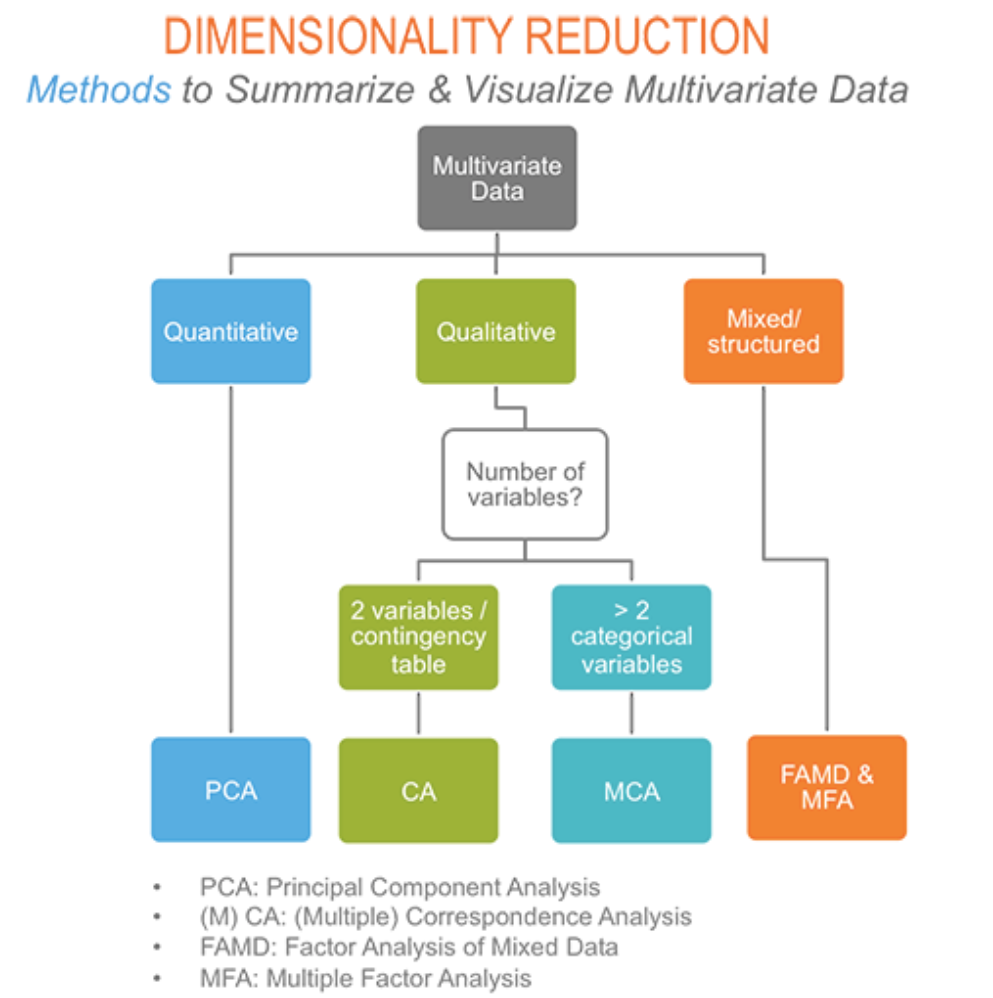
\includegraphics[width=0.6\textwidth,height=\textheight]{MCA,CA.png}
\caption{© Kassambara, 2017}
\end{figure}

\hypertarget{cloud-of-individuals-in-mca}{%
\section{Cloud of individuals in MCA}\label{cloud-of-individuals-in-mca}}

In the contingency table, individuals are shown as rows, thus, cloud of individuals are also called as points of rows. The distance between individuals of the cloud are determined by the responses to the categories of given questions, according how they answered differently. In MCA data presentation, it is also possible to present the cloud of individuals in accordance with the group of category in which the each point of individual belongs. Additionally, it enables to observe the outliers and individuals having similar characteristics which might help interpretation of the dataset.
In the example of data called ``poison'', cloud of individuals are shown as follows.

\begin{Shaded}
\begin{Highlighting}[]
\KeywordTok{data}\NormalTok{(poison)}
\NormalTok{poison.active <-}\StringTok{ }\NormalTok{poison[}\DecValTok{1}\OperatorTok{:}\DecValTok{55}\NormalTok{, }\DecValTok{5}\OperatorTok{:}\DecValTok{15}\NormalTok{]}
\NormalTok{res.mca4 <-}\StringTok{ }\KeywordTok{MCA}\NormalTok{(poison.active, }\DataTypeTok{graph =} \OtherTok{FALSE}\NormalTok{)}
\KeywordTok{fviz_mca_ind}\NormalTok{(res.mca4, }\DataTypeTok{col.ind =} \StringTok{"cos2"}\NormalTok{, }
             \DataTypeTok{gradient.cols =} \KeywordTok{c}\NormalTok{(}\StringTok{"#00AFBB"}\NormalTok{, }\StringTok{"#E7B800"}\NormalTok{, }\StringTok{"#FC4E07"}\NormalTok{),}
             \DataTypeTok{repel =} \OtherTok{TRUE}\NormalTok{, }
             \DataTypeTok{ggtheme =} \KeywordTok{theme_minimal}\NormalTok{())}
\end{Highlighting}
\end{Shaded}

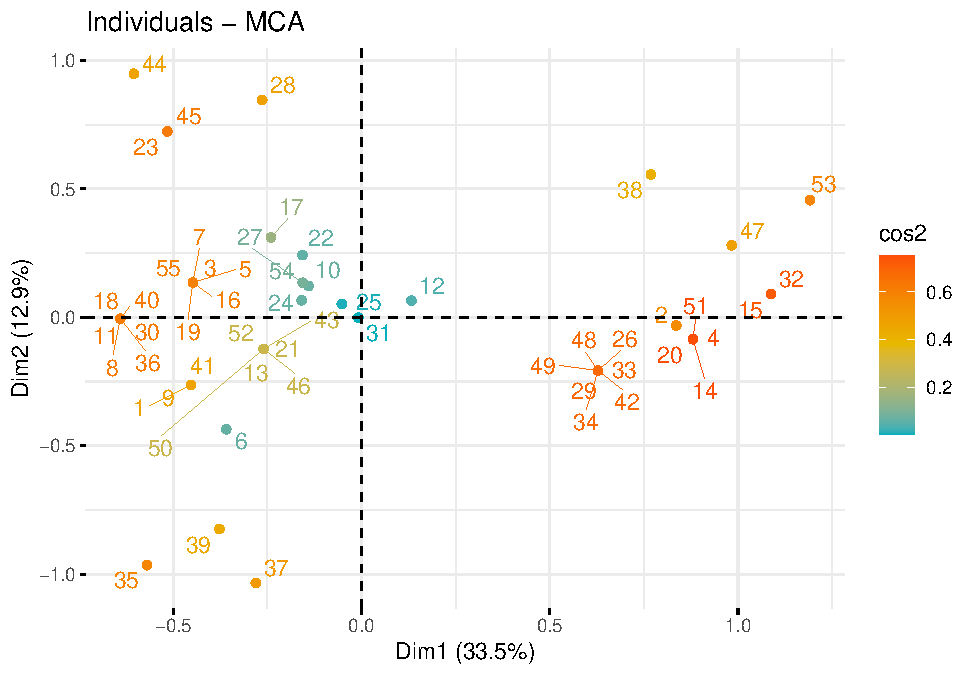
\includegraphics[width=0.6\linewidth]{Bookdown-MarinaObata2_files/figure-latex/4-2-1}

\hypertarget{cloud-of-categories-in-mca}{%
\section{Cloud of categories in MCA}\label{cloud-of-categories-in-mca}}

In the contingency table, categories are shown as columns, thus, cloud of categories are describing the clouds of columns of the dataset. The weight of a category is proportional to how common it is in the data, thus, in MCA, uncommon categories are located far from origins, the categories having similar characteristics are locating close to each other.
In the example of data ``poison'', cloud of categories are shown as follows. In this example, category ``Ice cream\_no'' and ``Potato\_no'' are locating far, therefore, could be considered as uncommon in the given dimension.

\begin{Shaded}
\begin{Highlighting}[]
\KeywordTok{fviz_mca_var}\NormalTok{(res.mca4, }
             \DataTypeTok{repel =} \OtherTok{TRUE}\NormalTok{, }
             \DataTypeTok{ggtheme =} \KeywordTok{theme_minimal}\NormalTok{())}
\end{Highlighting}
\end{Shaded}

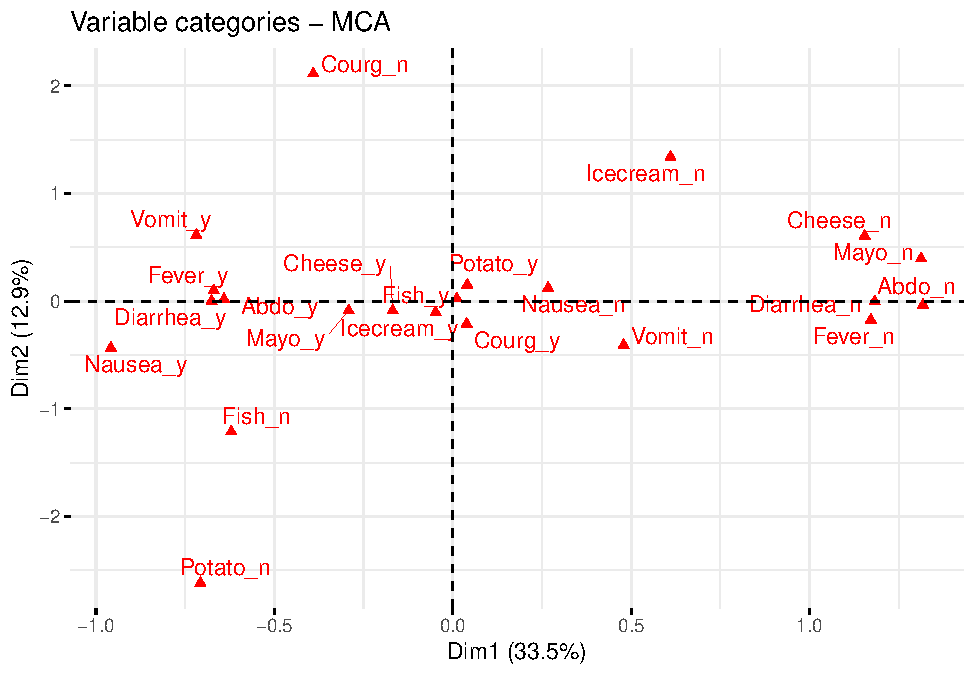
\includegraphics[width=0.6\linewidth]{Bookdown-MarinaObata2_files/figure-latex/4-3-1}

\hypertarget{prouxfb01le}{%
\section{Profile}\label{prouxfb01le}}

Profile means how the individual are related to the categories, if they have similar answer patterns towards categories, these individuals are close to each other, having a similar profile, if they answered very differently, these individuals locate farther apart.
In the example of data ``poison'', a group of individuals {[}26, 29, 33, 34, 42, 48, 49{]} is considered as having a similar profile in the given dimensions.

\begin{Shaded}
\begin{Highlighting}[]
\KeywordTok{fviz_mca_biplot}\NormalTok{(res.mca4, }
               \DataTypeTok{repel =} \OtherTok{TRUE}\NormalTok{,}
               \DataTypeTok{ggtheme =} \KeywordTok{theme_minimal}\NormalTok{())}
\end{Highlighting}
\end{Shaded}

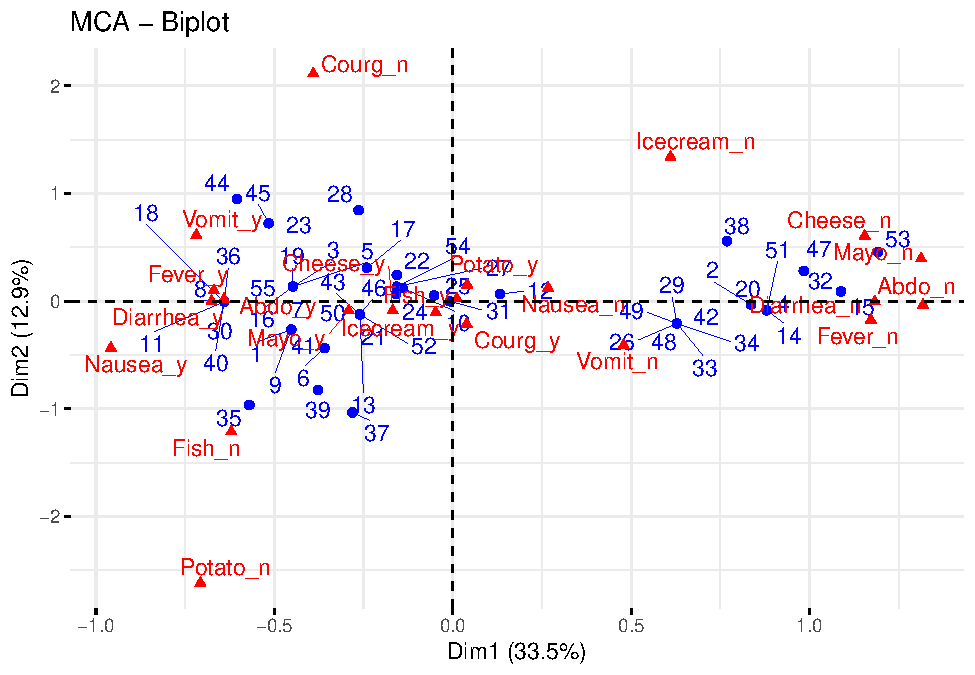
\includegraphics[width=0.6\linewidth]{Bookdown-MarinaObata2_files/figure-latex/4-4-1}

\hypertarget{weight}{%
\section{Weight}\label{weight}}

A weight is used in statistics in order to increase or decrease the importance of an item, this process is called as weighting. The weighting is used in MCA in order to balance measure of the similarity of the individuals against all the questions. In CA, the marginal values are used for weighting in order to give more or less importance to the display of the individual profiles regarding row and columns. As it is shown in the following example, the category `Modern art' and `Landscape' have rather similar contributions to axis 2, category Modern art has more distant from the center of axis 2 but smaller weight, however, category Landscape has less distant but more weighted.

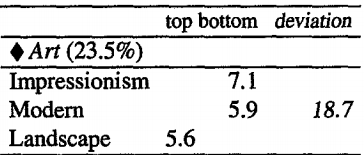
\includegraphics[width=0.5\textwidth,height=\textheight]{table MCA.png}
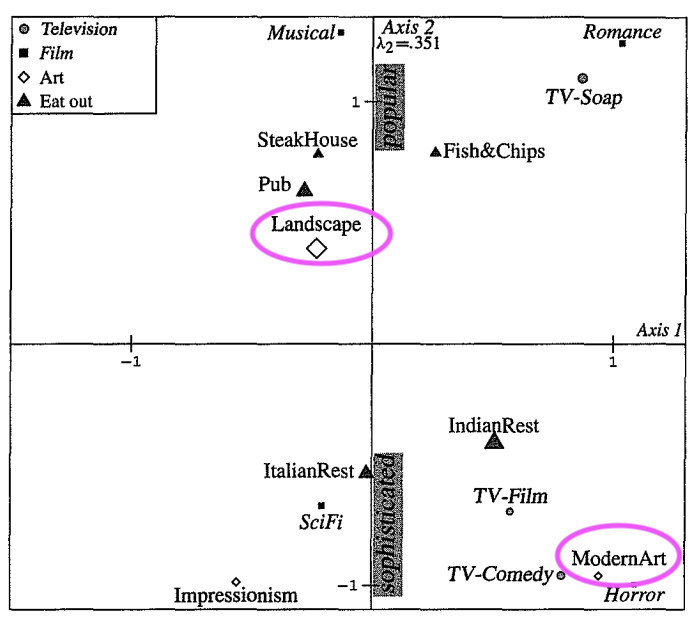
\includegraphics[width=0.5\textwidth,height=\textheight]{graph MCA.png}

\hypertarget{inertia}{%
\section{Inertia}\label{inertia}}

Inertia is the value which counts the distance of clouds of points in MCA. If the category has less frequency or having higher variance, the inertia gets higher. The total inertia which is a multidimensional extension of the concept of variance is defined as the sum of the squared distances from individuals to the center of gravity, weighted by the weight of the individuals.
It is different from PCA since inertia, which counts for constructing the distance in MCA is related to constructing dimensions in PCA.

\hypertarget{chi-square-distance}{%
\section{Chi-Square-Distance}\label{chi-square-distance}}

Both MCA and CA depends on the contingency tables, a commonway of describing the relationships in contingency table is the chi-square statistic, which tests for significant associations between rows and columns.
Chi-Square-Distance shows the similarity between two row profiles, which are the individuals and between column profiles of a two-way table. When Chi-Square shows the low value, it means there is a high correlation in between since it rejects the Null hypothesis of the rows and columns are independent. As a remark, in comparison to PCA, CA uses Chi-square value in stead of total variance when testing the independence. In MCA, the chi-squared distance is used as well since MCA is presented as a CA of the Burt matrix (explained in 5.13'Burt matrix').

\hypertarget{contribution}{%
\section{Contribution}\label{contribution}}

Contribution means how the elements are contributed in drawing MCA/CA, it depends both on the distance from the point to the origin point along the axis and on the weight of the point. It plays an important role for interpretation. If the category lies outside the confidence circle which locates in the middle of observations, having high variance, it could be considered contributing to the dependency, however, if it lies within the circle, the contribution seems low.
In the example of data ``poison'', following barplots are showing the contribution of variable categories. If we compare the barplot of dimension 2 and summary of data ``poison'', , the categories which have low frequency is showing the higher contribution, however, it depends on the dimension.

\begin{Shaded}
\begin{Highlighting}[]
\KeywordTok{fviz_contrib}\NormalTok{(res.mca4, }\DataTypeTok{choice =} \StringTok{"var"}\NormalTok{, }\DataTypeTok{axes =} \DecValTok{1}\NormalTok{, }\DataTypeTok{top =} \DecValTok{15}\NormalTok{)}
\end{Highlighting}
\end{Shaded}

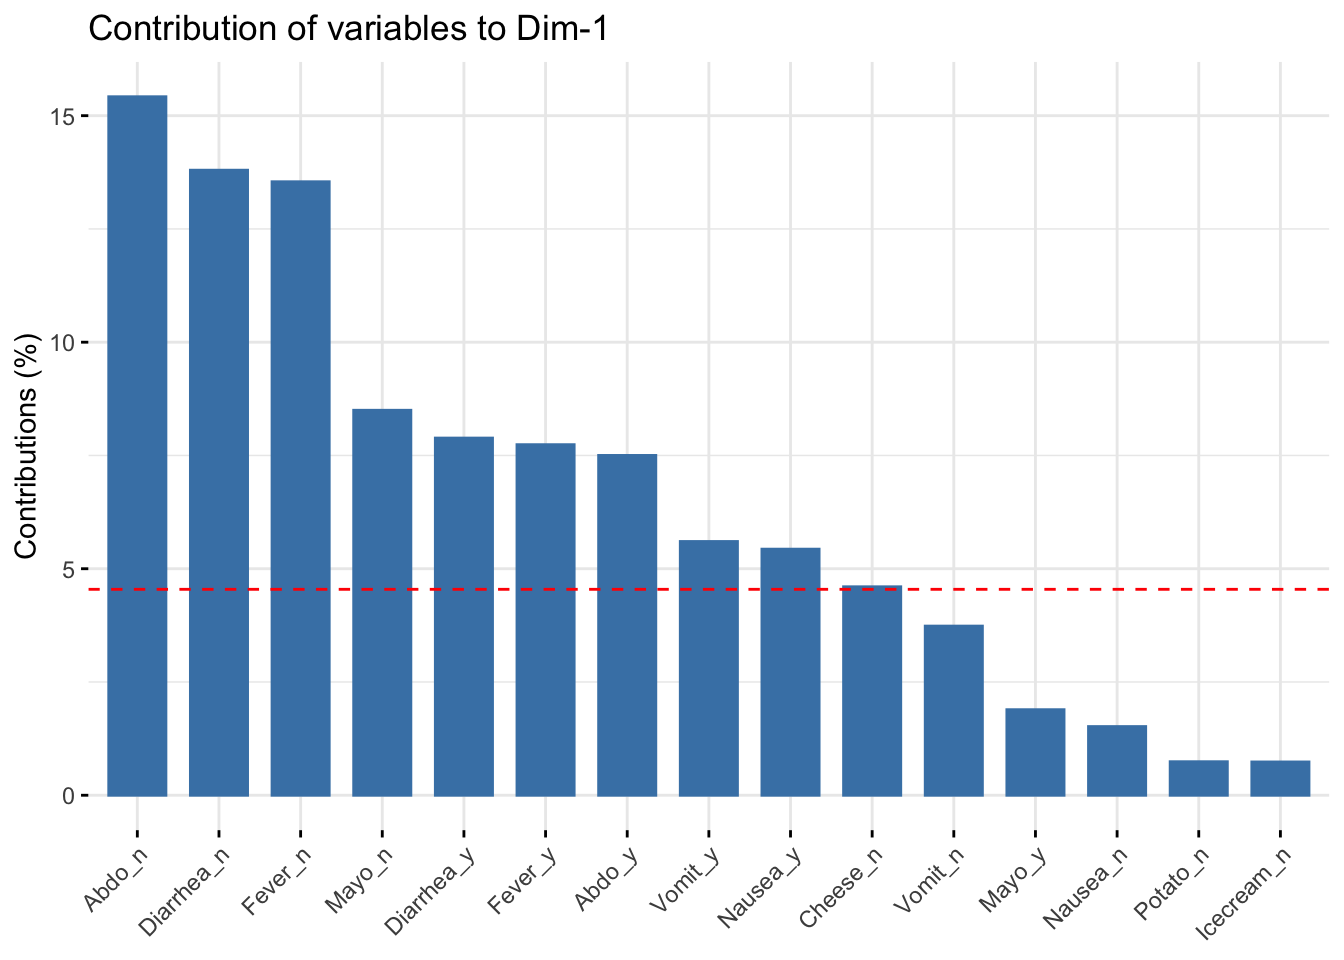
\includegraphics[width=0.5\linewidth]{Bookdown-MarinaObata2_files/figure-latex/4-5-1}

\begin{Shaded}
\begin{Highlighting}[]
\KeywordTok{fviz_contrib}\NormalTok{(res.mca4, }\DataTypeTok{choice =} \StringTok{"var"}\NormalTok{, }\DataTypeTok{axes =} \DecValTok{2}\NormalTok{, }\DataTypeTok{top =} \DecValTok{15}\NormalTok{)}
\end{Highlighting}
\end{Shaded}

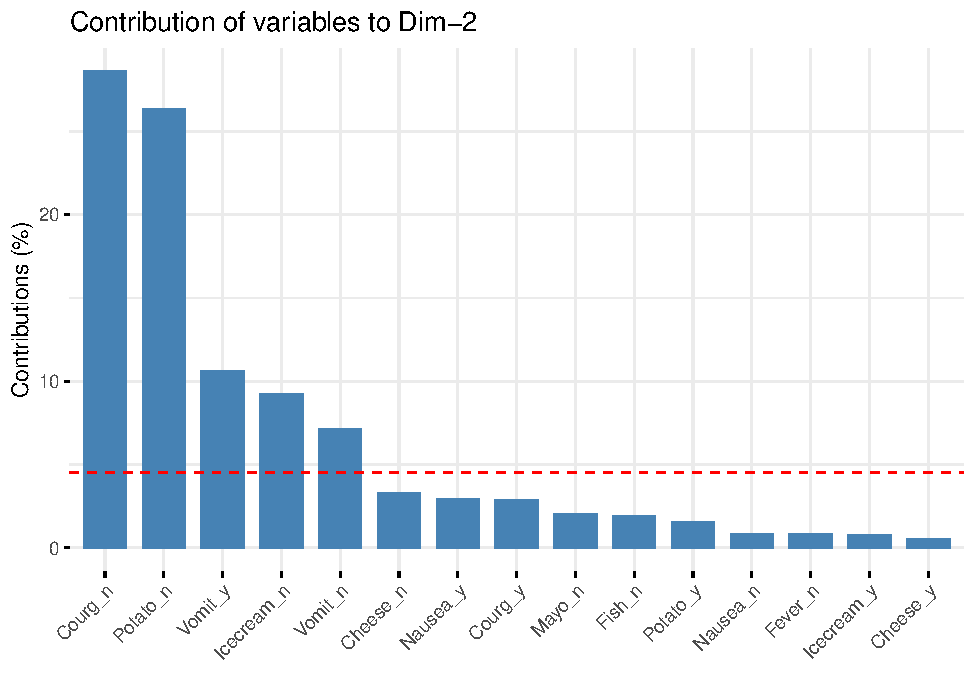
\includegraphics[width=0.5\linewidth]{Bookdown-MarinaObata2_files/figure-latex/4-5-2}

\begin{Shaded}
\begin{Highlighting}[]
\KeywordTok{summary}\NormalTok{(poison)}
\end{Highlighting}
\end{Shaded}

\begin{verbatim}
##       Age             Time           Sick    Sex         Nausea      Vomiting 
##  Min.   : 4.00   Min.   : 0.00   Sick_n:17   F:28   Nausea_n:43   Vomit_n:33  
##  1st Qu.: 6.00   1st Qu.: 0.00   Sick_y:38   M:27   Nausea_y:12   Vomit_y:22  
##  Median : 8.00   Median :12.00                                                
##  Mean   :16.93   Mean   :10.16                                                
##  3rd Qu.:10.00   3rd Qu.:16.50                                                
##  Max.   :88.00   Max.   :22.00                                                
##   Abdominals     Fever          Diarrhae       Potato       Fish        Mayo   
##  Abdo_n:18   Fever_n:20   Diarrhea_n:20   Potato_n: 3   Fish_n: 1   Mayo_n:10  
##  Abdo_y:37   Fever_y:35   Diarrhea_y:35   Potato_y:52   Fish_y:54   Mayo_y:45  
##                                                                                
##                                                                                
##                                                                                
##                                                                                
##    Courgette       Cheese         Icecream 
##  Courg_n: 5   Cheese_n: 7   Icecream_n: 4  
##  Courg_y:50   Cheese_y:48   Icecream_y:51  
##                                            
##                                            
##                                            
## 
\end{verbatim}

\hypertarget{supplementary-variablesindividuals-in-camca}{%
\section{Supplementary variables/individuals in CA/MCA}\label{supplementary-variablesindividuals-in-camca}}

Supplementary variables/individuals are in contrast to the active individuals/variables which are used for the determination of the MCA/CA, not participating them, however, it may help to interpret the data. Their coordinates are predicted by using only the information provided by the performed MCA/CA on active individuals/variables. It is also possible to highlight the correlation between active and supplementary variables and dimensions in MCA/CA, however, supplementary variables/individuals don't contribute to the construction of the axes.
In the example of data ``poison'', the supplementary variables are ``time'' and ``age'', supplementary individuals are {[}53, 54, 55{]}.

\begin{Shaded}
\begin{Highlighting}[]
\KeywordTok{MCA}\NormalTok{(poison, }\DataTypeTok{ind.sup =} \DecValTok{53}\OperatorTok{:}\DecValTok{55}\NormalTok{, }
               \DataTypeTok{quanti.sup =} \DecValTok{1}\OperatorTok{:}\DecValTok{2}\NormalTok{, }\DataTypeTok{quali.sup =} \DecValTok{3}\OperatorTok{:}\DecValTok{4}\NormalTok{,  }\DataTypeTok{graph=}\OtherTok{TRUE}\NormalTok{)}
\end{Highlighting}
\end{Shaded}

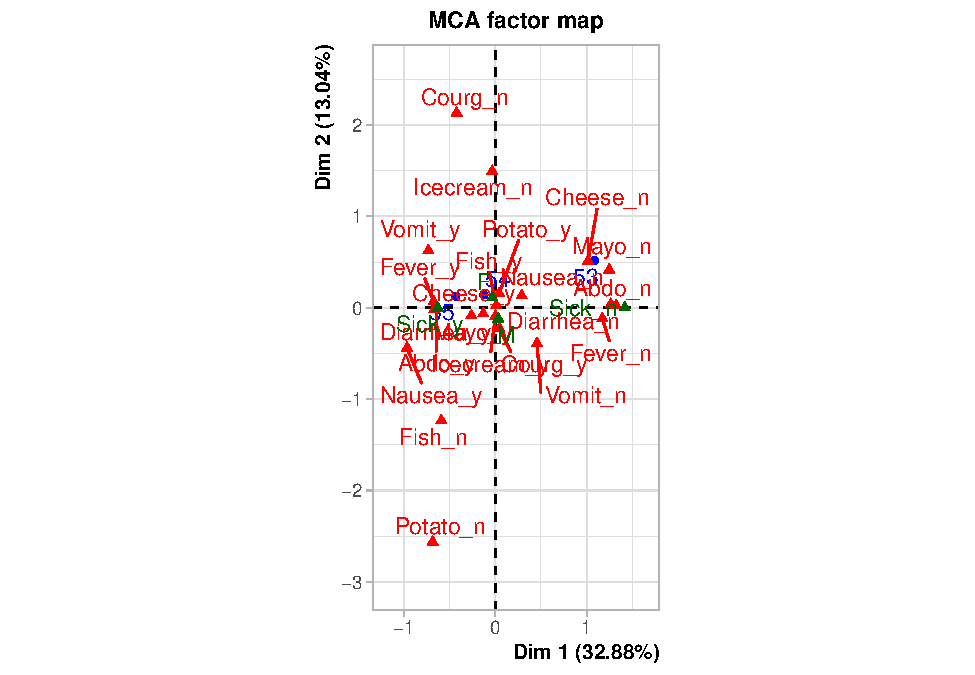
\includegraphics[width=0.5\linewidth]{Bookdown-MarinaObata2_files/figure-latex/4-6-1}
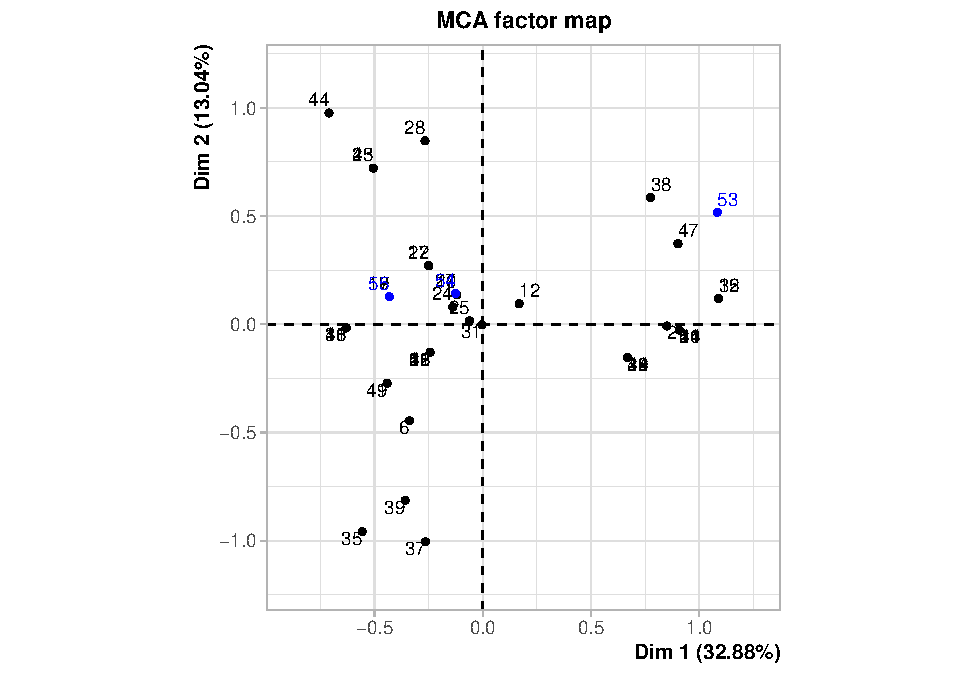
\includegraphics[width=0.5\linewidth]{Bookdown-MarinaObata2_files/figure-latex/4-6-2}
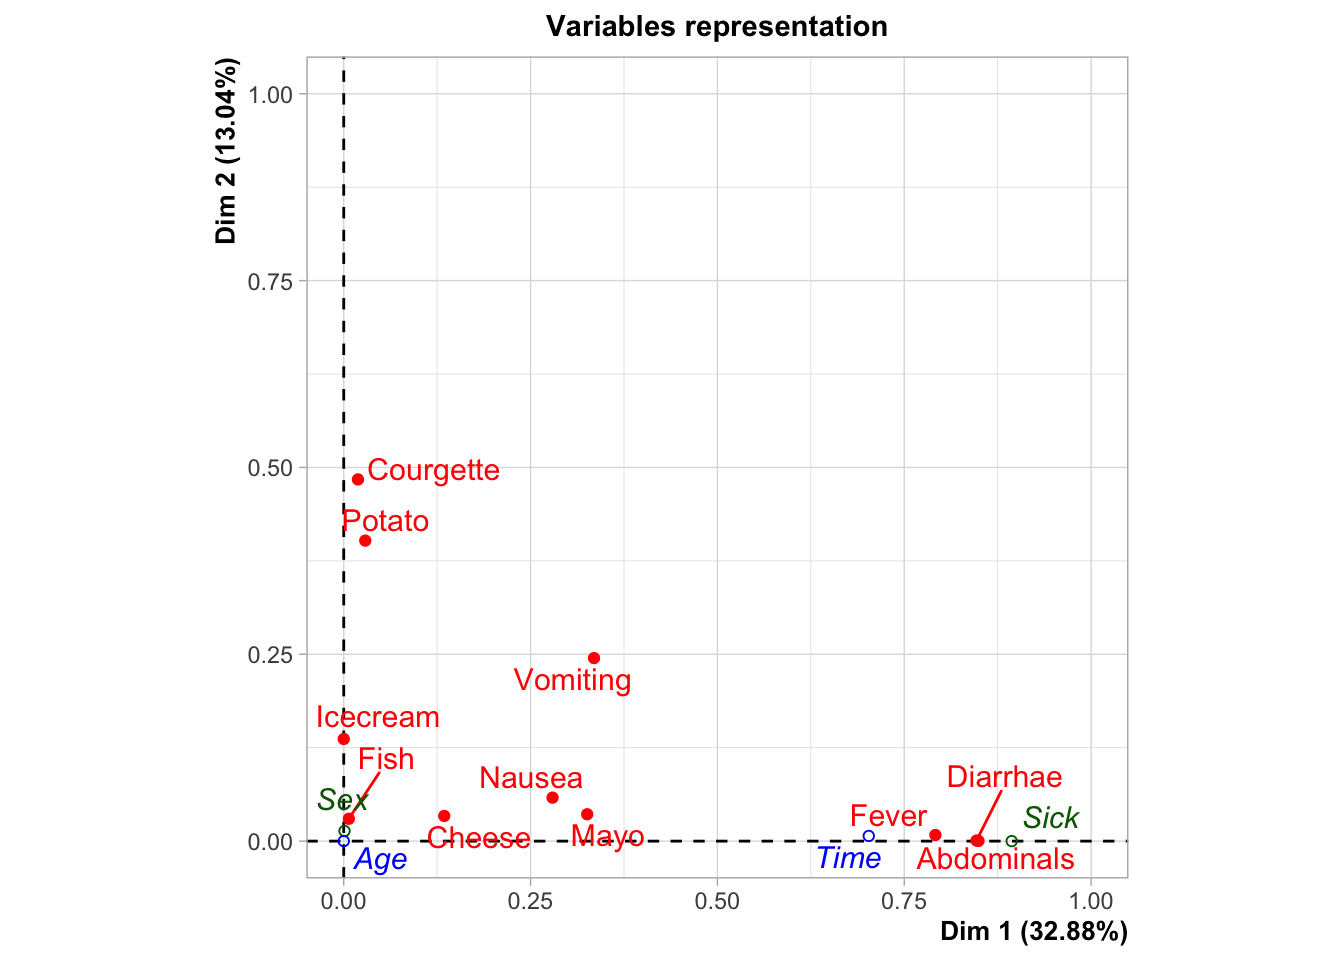
\includegraphics[width=0.5\linewidth]{Bookdown-MarinaObata2_files/figure-latex/4-6-3}
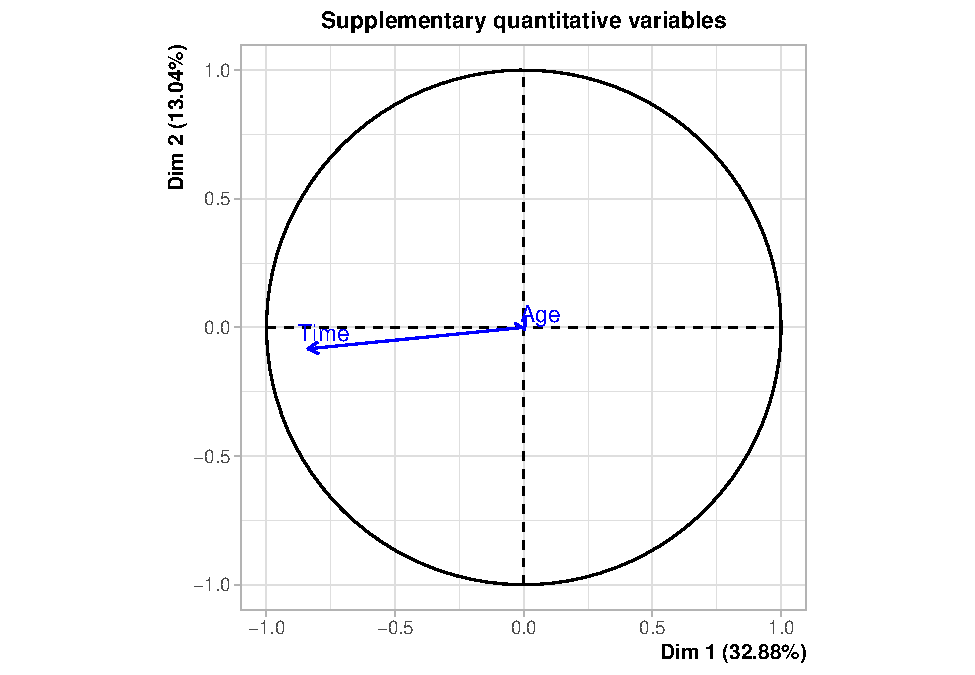
\includegraphics[width=0.5\linewidth]{Bookdown-MarinaObata2_files/figure-latex/4-6-4}

quasi.sup' and `quail.sup' are specifying the indexes of quantitative and qualitative variables. `ind.sup' is the numeric vector, specifying the indexes of the supplementary individuals.

\hypertarget{concentration-ellipse}{%
\section{Concentration ellipse}\label{concentration-ellipse}}

Concentration ellipse provides geometric summaries of subclouds, for a normally shaped cloud, the concentration ellipse sums up plus, minus 2 standard divination in a two-dimensional distribution, containing about 86\% of the points of the cloud. As an example, it allows to examine the dispersion of individuals belonging to particular or supplementary categories.

\begin{Shaded}
\begin{Highlighting}[]
\NormalTok{grp <-}\StringTok{ }\KeywordTok{as.factor}\NormalTok{(poison.active[, }\StringTok{"Vomiting"}\NormalTok{])}
\KeywordTok{fviz_mca_ind}\NormalTok{(res.mca4, }\DataTypeTok{habillage=}\NormalTok{grp,}
             \DataTypeTok{addEllipses=}\OtherTok{TRUE}\NormalTok{)}
\end{Highlighting}
\end{Shaded}

\begin{figure}
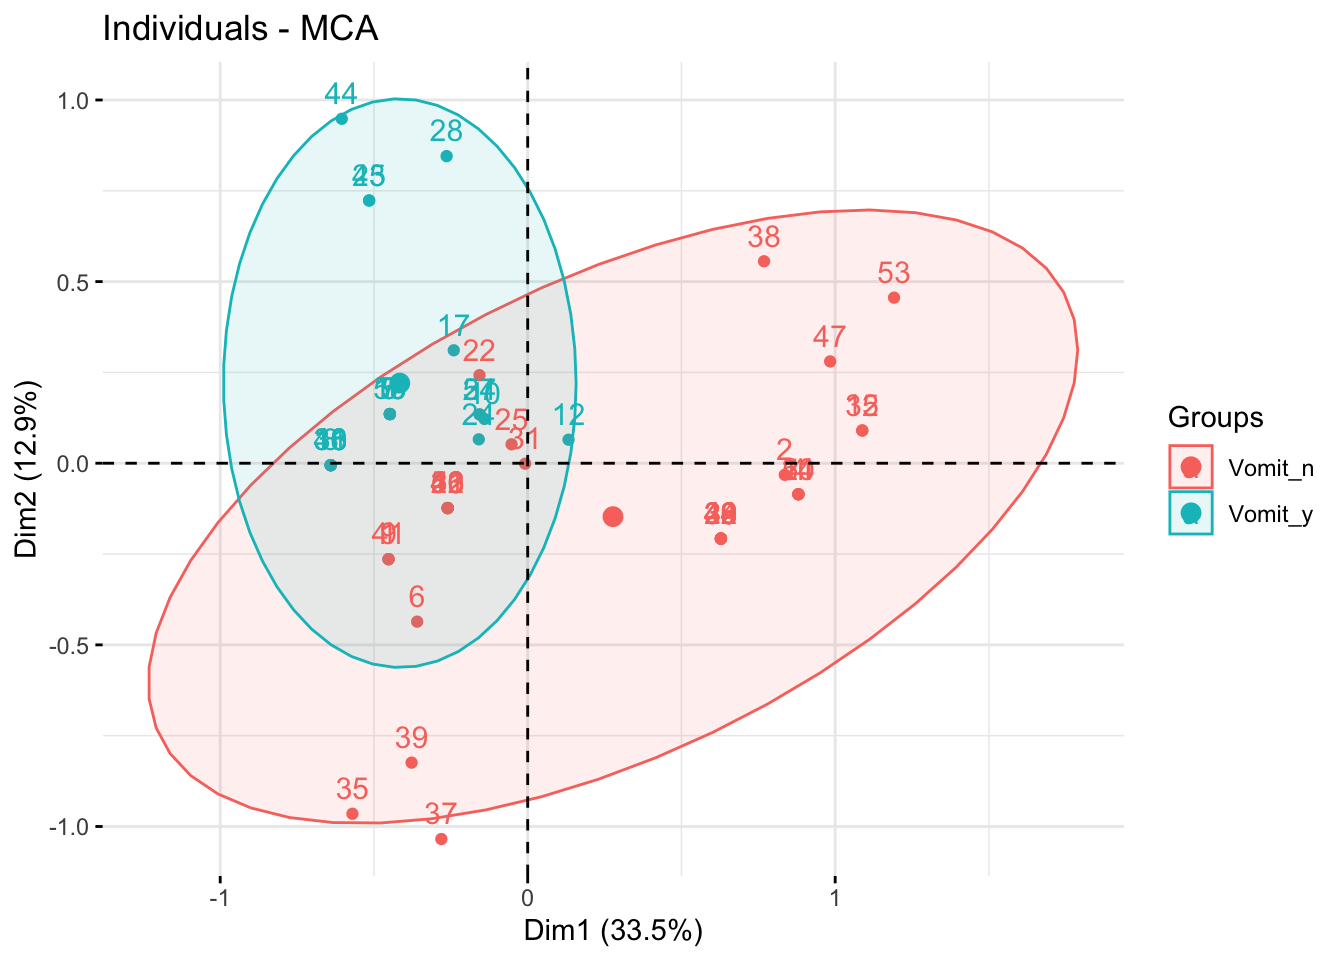
\includegraphics[width=0.6\linewidth]{Bookdown-MarinaObata2_files/figure-latex/4-7-1} \caption{An example of confidence ellipse}\label{fig:4-7}
\end{figure}

\hypertarget{confidence-ellipse}{%
\section{Confidence ellipse}\label{confidence-ellipse}}

Confidence ellipses shows the region that constrains the certain amount of (i.e.~95\%) confidence ellipses of all cloud of points which can be drawn from the MCA/CA. It plots the confidence ellipses around group mean point, as an example, it enables to visualize whether two categories differ significantly.

\begin{figure}
\centering
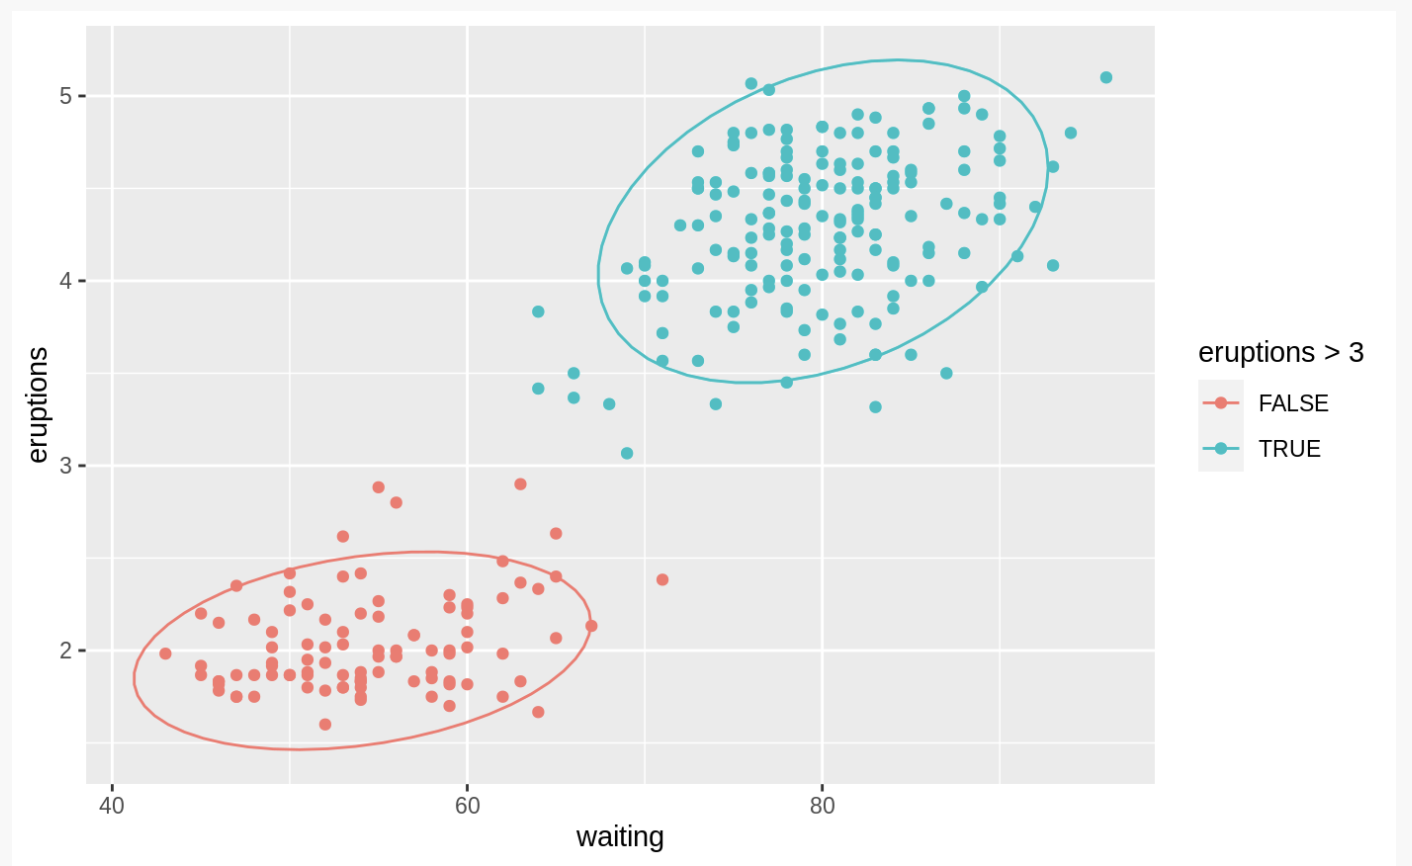
\includegraphics[width=0.5\textwidth,height=\textheight]{confident ellipse.png}
\caption{© Kassambara, 2017}
\end{figure}

\hypertarget{binary-indicator-matrix}{%
\section{Binary indicator matrix}\label{binary-indicator-matrix}}

Binary indicator matrix has only the values 0 and 1, the individuals/groups are listed as rows, the categories are listed as columns. Thus, the number of rows are the total sample items, and the columns are the total categories of the variables. If the item is corresponding to the category of the variable, the elements in the indicator matrix shows 1, if not, it shows 0. This indicator matrix helps to see the characteristics of the cloud simply, at the same time, to consider the distances in between.

\begin{figure}
\centering
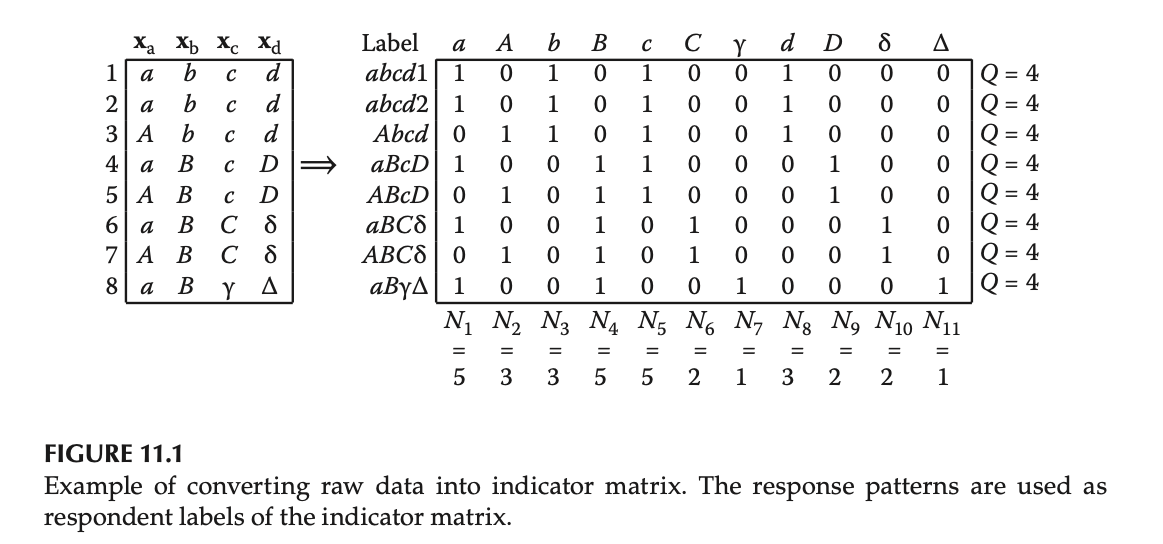
\includegraphics[width=0.7\textwidth,height=\textheight]{IDM.png}
\caption{© Husson, 2014}
\end{figure}

\hypertarget{burt-matrix}{%
\section{Burt matrix}\label{burt-matrix}}

Burt matrix is assembling all the relevant cross-tables into a square super matrix of cross-tables in CA. It includes the diagonal associations between each variables and itself. Only the information about the relationship between categories are included, however, it is possible to present the information about individuals on the graph by projecting the indicator matrix as supplementary elements. `Z' from the figure below is often called matrix of dummy variables, the elements of Z are zeros except for the ones indicating the categories of response of each respondent. MCA is a method that the usual CA algorithm is applied to a burt matrix.

\begin{figure}
\centering
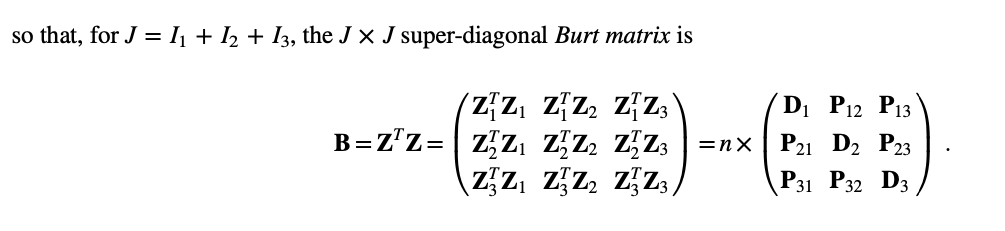
\includegraphics[width=0.7\textwidth,height=\textheight]{burt matrix.png}
\caption{© Beh and Lombardo, 2019}
\end{figure}

\hypertarget{references-3}{%
\section{References}\label{references-3}}

Beh.E.J. and Lombardo.R. (2019).Multiple and multiway correspondence analysis. Wiley Online Library. {[}online{]}. Retrieved from \url{https://onlinelibrary.wiley.com/doi/abs/10.1002/wics.1464} {[}accessed on 15.06.2020{]}.

Costa.P.S., Santos.N.C., Cunha.P., Cotter.J. and Sousa. Nuno. (2013).The Use of Multiple Correspondence Analysis to Explore Associations between Categories of Qualitative Variables in Healthy Ageing. Journal of Asing Research. {[}online{]}.Retrieved from \url{https://www.hindawi.com/journals/jar/2013/302163/} {[}accessed on 15.06.2020{]}.

Greenacre.M. and Blasius.J.(2006).Multiple Correspondence Analysis and Related Methods.Chapman \& Hall/CRC.

Hjellbrekke. J. (2018). Multiple Correspondence Analysis for the Social Sciences. Routledge.

Husson.F.(2014). Multiple Correspondence Analysis.The Visualization and Verbalization of DataChapter: Multiple Correspondence Analysis.CRC/PRESS.

Husson.F., Lê. S. and Pagès. J. (2017).Exploratory Multivariate Analysis by Example Using R. Second edition. Chapman \& Hall/CRC.

Kassambara.A. (2017). Articles - Principal Component Methods in R: Practical Guide. CA - Correspondence Analysis in R: Essentials. {[}online{]}. Retrieved from \url{http://www.sthda.com/english/articles/31-principal-component-methods-in-r-practical-guide/113-ca-correspondence-analysis-in-r-essentials/} {[}accessed on 15.06.2020{]}.

Kassambara.A. (2017). Articles - Principal Component Methods in R: Practical Guide. MCA - Multiple Correspondence Analysis in R: Essentials. Statistical tool for high-thoughtput data analysis. {[}online{]}. Retrieved from \url{http://www.sthda.com/english/articles/31-principal-component-methods-in-r-practical-guide/114-mca-multiple-correspondence-analysis-in-r-essentials/} {[}accessed on 15.06.2020{]}

Kassambara.A. (2017). Practical Guide To Cluster Analysis in R. sthda.com . Edition 1.

Le Roux.B.and Rouanet.H. (2004). Geometric Data Analysis. Kluwer Academic Publishers.

Le Roux.B. and Rouanet.H. (2010).Multiple Correspondence Analysis.Sage Publications.

\hypertarget{glossary-5-cluster-analysis}{%
\chapter{Glossary 5 (Cluster Analysis)}\label{glossary-5-cluster-analysis}}

\hypertarget{euclidean-distance}{%
\section{Euclidean distance}\label{euclidean-distance}}

In cluster analysis, the proximities between individuals are quantified by distance measures, Euclidean distance measure is the most commonly used one, it used to assign points to clusters. It treats each variable as equally important when calculating the distance, usually computed from raw data, not from standardized data. In order to calculate the Euclidean distance, the sum of squared distances of adjoining side(B), opposite side(A) of the hypotenuse(C) are square rooted (sqrt(A\^{}2 + B\^{}2), see the image below). If Euclidean distance is chosen, the observations with high values of features will be clustered together, so will be for the observations with low values of features.

\begin{figure}
\centering
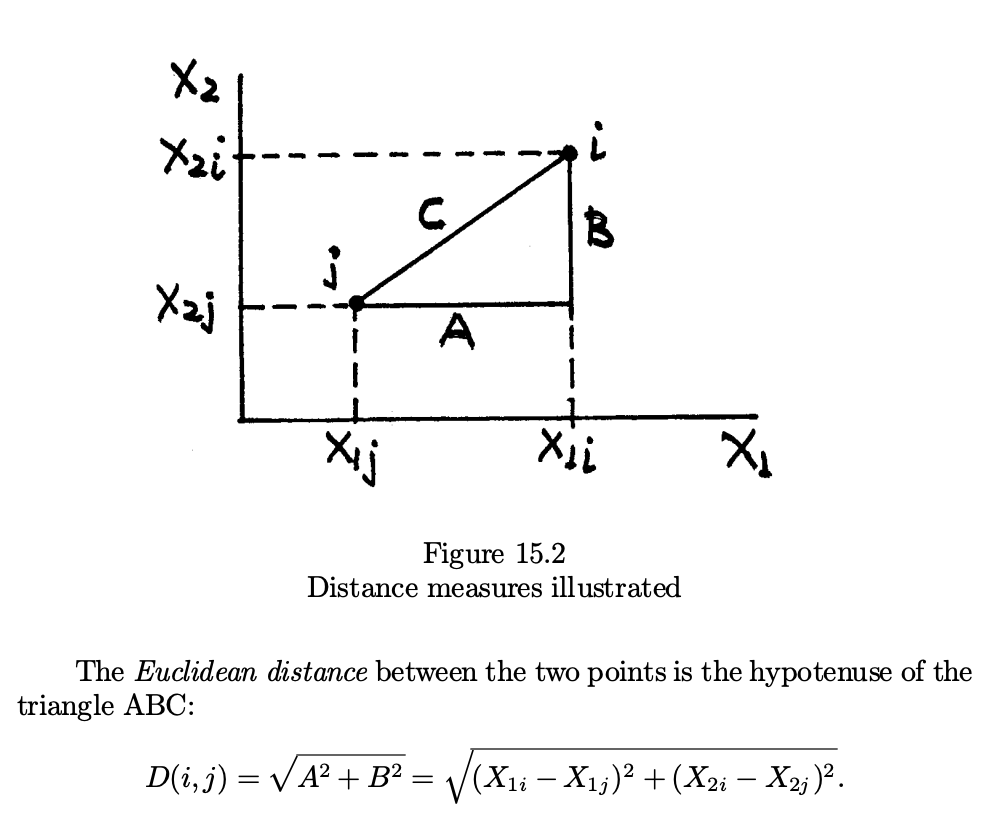
\includegraphics[width=0.5\textwidth,height=\textheight]{Euclidean.png}
\caption{© Tryfos, 2001}
\end{figure}

Following matrix table shows an example of Euclidean distance from the data of arrested record in the U.S.

\begin{Shaded}
\begin{Highlighting}[]
\KeywordTok{set.seed}\NormalTok{(}\DecValTok{123}\NormalTok{)}
\NormalTok{ss <-}\StringTok{ }\KeywordTok{sample}\NormalTok{(}\DecValTok{1}\OperatorTok{:}\DecValTok{50}\NormalTok{, }\DecValTok{15}\NormalTok{)}
\NormalTok{df5 <-}\StringTok{ }\NormalTok{USArrests[ss, ] }
\NormalTok{df.scaled <-}\StringTok{ }\KeywordTok{scale}\NormalTok{(df5) }
\NormalTok{dist.eucl <-}\StringTok{ }\KeywordTok{dist}\NormalTok{(df.scaled, }\DataTypeTok{method =} \StringTok{"euclidean"}\NormalTok{)}
\KeywordTok{round}\NormalTok{(}\KeywordTok{as.matrix}\NormalTok{(dist.eucl)[}\DecValTok{1}\OperatorTok{:}\DecValTok{3}\NormalTok{, }\DecValTok{1}\OperatorTok{:}\DecValTok{3}\NormalTok{], }\DecValTok{1}\NormalTok{)}
\end{Highlighting}
\end{Shaded}

\begin{verbatim}
##            New Mexico Iowa Indiana
## New Mexico        0.0  4.1     2.5
## Iowa              4.1  0.0     1.8
## Indiana           2.5  1.8     0.0
\end{verbatim}

\hypertarget{manhattan-distance}{%
\section{Manhattan distance}\label{manhattan-distance}}

Manhattan distance captures the distance by aggregating the pairwise absolute difference between each variable. It follows a route along the non-hypotenuse sides of a triangle. The name of Manhattan is referring the grid-like layout of most American cities in which it is hard to go directly between two points. The difference between Euclidean distance is that it is not using the squared distance, just summing the absolute numbers(see the image below). Manhattan distance is less sensitive to outliers when applied to cluster analysis.

\[
d(i.j) = \sum|Xik-Xjk|
\]

\begin{figure}
\centering
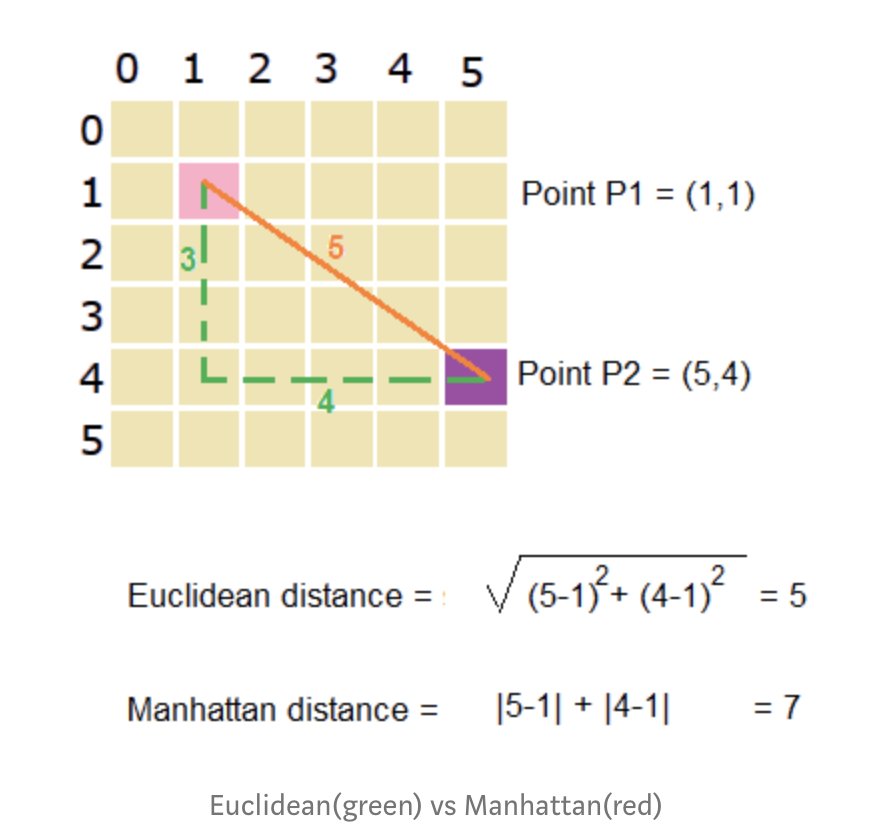
\includegraphics[width=0.4\textwidth,height=\textheight]{Manhattan.png}
\caption{© Chatterjee, 2019}
\end{figure}

Following matrix table shows an example of Euclidean distance. As you can see, even though the used data is the same, it shows different values from Euclidean distance, having larger distances.

\begin{Shaded}
\begin{Highlighting}[]
\NormalTok{dist.manh <-}\StringTok{ }\KeywordTok{dist}\NormalTok{(df.scaled, }\DataTypeTok{method =} \StringTok{"manhattan"}\NormalTok{)}
\KeywordTok{round}\NormalTok{(}\KeywordTok{as.matrix}\NormalTok{(dist.manh)[}\DecValTok{1}\OperatorTok{:}\DecValTok{3}\NormalTok{, }\DecValTok{1}\OperatorTok{:}\DecValTok{3}\NormalTok{], }\DecValTok{1}\NormalTok{)}
\end{Highlighting}
\end{Shaded}

\begin{verbatim}
##            New Mexico Iowa Indiana
## New Mexico        0.0  7.8     4.4
## Iowa              7.8  0.0     3.4
## Indiana           4.4  3.4     0.0
\end{verbatim}

\hypertarget{mahalanobis-distance}{%
\section{Mahalanobis distance}\label{mahalanobis-distance}}

The Mahalanobis distance is an approach to scale the distance in accordance with the variability of each variable. In the K-means algorithm, the Mahalanobis distance metric could be used to capture the variance structure of the clusters, it allows K-means to identify non-homogeneous clusters. When correlations between variables within groups are small, Mahalanobis distance will be similar as squared Euclidean distance. Which means, Mahalanobis distance increases when the distance of centers between two groups increases, it decreases when there are larger variations within the group. It is suggested by Kurczynski(1969) to adapt the generalized Mahalanobis distance with categorical variables.

\begin{figure}
\centering
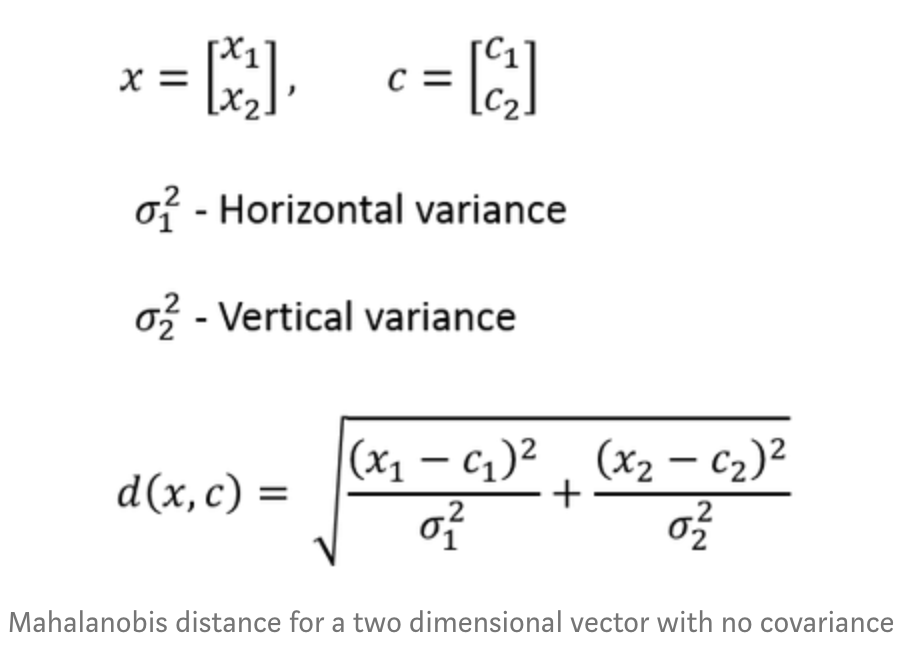
\includegraphics[width=0.4\textwidth,height=\textheight]{Mahala.png}
\caption{© Chatterjee, 2019}
\end{figure}

The following calculation is showing the mahalanobis distance from the same data of arrested record in the U.S.

\begin{Shaded}
\begin{Highlighting}[]
\NormalTok{dist.mahala <-}\StringTok{ }\KeywordTok{distances}\NormalTok{(df.scaled, }\DataTypeTok{normalize =} \StringTok{"mahalanobize"}\NormalTok{)}
\NormalTok{df.n <-}\StringTok{ }\KeywordTok{round}\NormalTok{(}\KeywordTok{as.matrix}\NormalTok{(dist.mahala)[}\DecValTok{1}\OperatorTok{:}\DecValTok{3}\NormalTok{, }\DecValTok{1}\OperatorTok{:}\DecValTok{3}\NormalTok{], }\DecValTok{1}\NormalTok{)}
\KeywordTok{rownames}\NormalTok{(df.n) <-}\StringTok{ }\KeywordTok{c}\NormalTok{(}\StringTok{"New Mexico"}\NormalTok{, }\StringTok{"Iowa"}\NormalTok{, }\StringTok{"Indiana"}\NormalTok{)}
\KeywordTok{colnames}\NormalTok{(df.n) <-}\StringTok{ }\KeywordTok{c}\NormalTok{(}\StringTok{"New Mexico"}\NormalTok{, }\StringTok{"Iowa"}\NormalTok{, }\StringTok{"Indiana"}\NormalTok{)}
\NormalTok{df.n }
\end{Highlighting}
\end{Shaded}

\begin{verbatim}
##            New Mexico Iowa Indiana
## New Mexico        0.0  2.9     2.5
## Iowa              2.9  0.0     1.6
## Indiana           2.5  1.6     0.0
\end{verbatim}

As it is mentioned, it is closer to Euclidean distance than Manhattan distance in this example.

\hypertarget{hierarchical-clustering}{%
\section{Hierarchical clustering}\label{hierarchical-clustering}}

Hierarchical clustering is one of the main categories of clustering techniques, it concerns a suitable choice of a distance function to express the distance and patterns. It is a statistical method for finding relatively homogeneous clusters, based on distances between objects. It reduces the number of clusters by combining the clusters having similar characteristics at each level till reach to only one cluster left (see the image below).

\begin{figure}
\centering
\includegraphics[width=0.4\textwidth,height=\textheight]{Hierarchical.png}
\caption{© Sinharay, 2010}
\end{figure}

\hypertarget{partitioning}{%
\section{Partitioning}\label{partitioning}}

Partitioning is a process in cluster analysis, grouping the similar observations into homogeneous subsets. For example, partitioning in hierarchical analysis means the process to combining the similar clusters at each level.
The Partitioning-based clustering is one of the major types of cluster analysis, Grabmeier and Rudolph's (2002) taxonomy separated partitioning methods from hierarchical methods. This method is based on interactive relocation of data points between clusters, the quality is measured by a clustering criterion. There are various types of partitioning clustering algorithms such as K-means, K-methods, FCM, CLARANS.
Among that, K-means requires the analyst to define K number of clusters before running the algorithm.

\hypertarget{dendrogram}{%
\section{Dendrogram}\label{dendrogram}}

Dendrogram is a type of tree shaped diagram showing the hierarchical clustering, it can visualize how close/far the clusters are to other clusters(see the figure below). Those clades with different heights are indicating how similar/dissimilar the clusters are, having same heights of clades meaning that they are similar to each other. Also, dendrogram is illustrating the process of divisions which have been made at each level of hierarchical analysis, it enables to decide the level at which to cut the tree for suitable number of clustering groups.
Following dendrogram shows the example data of arrested records in the U.S.

\begin{Shaded}
\begin{Highlighting}[]
\NormalTok{res.dist <-}\StringTok{ }\KeywordTok{dist}\NormalTok{(df5, }\DataTypeTok{method =} \StringTok{"euclidean"}\NormalTok{)}
\NormalTok{res.hc <-}\StringTok{ }\KeywordTok{hclust}\NormalTok{(}\DataTypeTok{d =}\NormalTok{ res.dist, }\DataTypeTok{method =} \StringTok{"ward.D2"}\NormalTok{)}
\KeywordTok{fviz_dend}\NormalTok{(res.hc, }\DataTypeTok{cex =} \FloatTok{0.5}\NormalTok{)}
\end{Highlighting}
\end{Shaded}

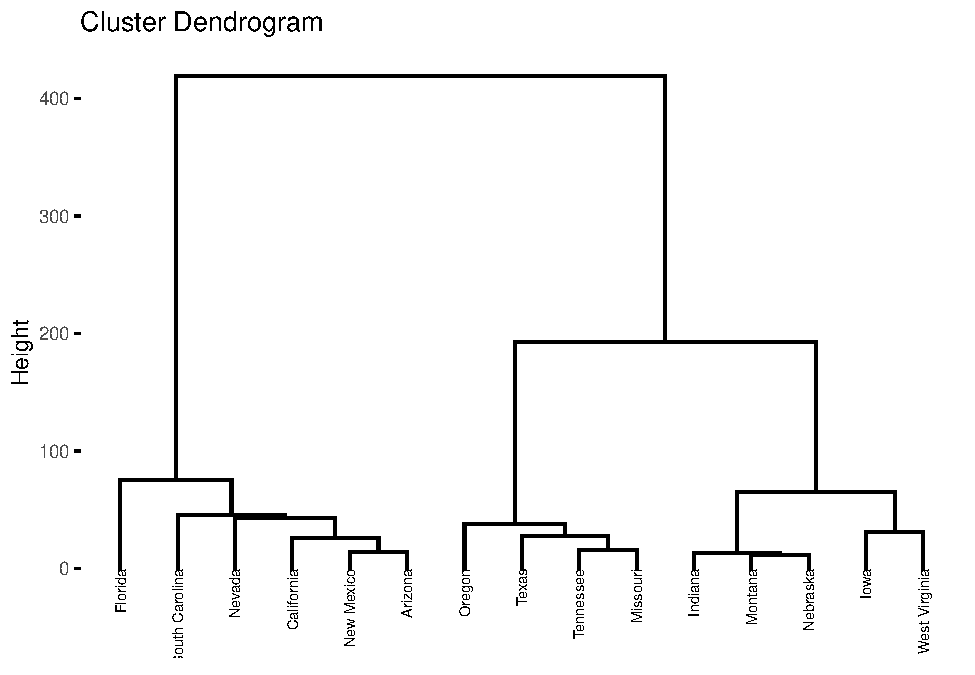
\includegraphics[width=0.6\linewidth]{Bookdown-MarinaObata2_files/figure-latex/5-5-1}

\hypertarget{references-4}{%
\section{References}\label{references-4}}

Chatterjee.D.R.(2019).Log Book --- Guide to Distance Measuring Approaches for K- Means Clustering. Towards data science. {[}online{]}.Retrieved from \url{https://towardsdatascience.com/log-book-guide-to-distance-measuring-approaches-for-k-means-clustering-f137807e8e21} {[}accessed on 15.06.2020{]}.

Deltaflair Team (2019). Clustering in R -- A Survival Guide on Cluster Analysis in R for Beginners{[}online{]}.Retrieved from \url{https://data-flair.training/blogs/clustering-in-r-tutorial/} {[}accessed on 15.06.2020{]}.

Kassambara.A. (2017).Articles - Cluster Analysis in R: Practical Guide. Essentials. Statistical tool for high-thoughtput data analysis. {[}online{]}. Retrieved from \url{http://www.sthda.com/english/articles/25-clusteranalysis-in-r-practical-guide/} {[}accessed on 15.06.2020{]}.

Kassambara.A. (2017). Practical Guide To Cluster Analysis in R. sthda.com . Edition 1.

Kassambara.A. (2017).Articles - Principal Component Methods in R: Practical Guide. Principal Component Analysis in R: prcomp vs princomp. {[}online{]}.Retrieved from \url{http://www.sthda.com/english/articles/31-principal-component-methods-in-r-practical-guide/118-principal-component-analysis-in-r-prcomp-vs-princomp/} {[}accessed on 15.06.2020{]}.

Le Roux.B.and Rouanet.H. (2004). Geometric Data Analysis. Kluwer Academic Publishers.

Nalson.J.(2012). ON K-means Clustering Using Mahalanobis Distance{[}onlone{]}. Retrieved from \url{https://pdfs.semanticscholar.org/b029/5854310ef3e35a0d71bd73554840e38a5bd8.pdf} {[}accessed on 16.06.2020{]}.

Savje.F. (2019). Package `distances'. CRAN.{[}online{]}.Retrieved from \url{https://cran.r-project.org/web/packages/distances/distances.pdf} {[}accessed on 15.06.2020{]}.
Sinharay.S.(2010).International Encyclopedia of Education (Third Edition).Cluster Analysis.

Tryfos.P.(1997). Chapter 15 Cluster analysis.{[}online{]}.Retrieved from \url{http://www.yorku.ca/ptryfos/f1500.pdf} {[}accessed on 15.06.2020{]}.

\bibliography{book.bib,packages.bib}

\end{document}
